\documentclass[12pt,a4paper]{article}

\usepackage[a4paper,text={16.5cm,25.2cm},centering]{geometry}
\usepackage{lmodern}
\usepackage{amssymb,amsmath}
\usepackage{bm}
\usepackage{graphicx}
\usepackage{microtype}
\usepackage{hyperref}
\setlength{\parindent}{0pt}
\setlength{\parskip}{1.2ex}

\hypersetup
       {   pdfauthor = { Marco Fasondini },
           pdftitle={ foo },
           colorlinks=TRUE,
           linkcolor=black,
           citecolor=blue,
           urlcolor=blue
       }




\usepackage{upquote}
\usepackage{listings}
\usepackage{xcolor}
\lstset{
    basicstyle=\ttfamily\footnotesize,
    upquote=true,
    breaklines=true,
    breakindent=0pt,
    keepspaces=true,
    showspaces=false,
    columns=fullflexible,
    showtabs=false,
    showstringspaces=false,
    escapeinside={(*@}{@*)},
    extendedchars=true,
}
\newcommand{\HLJLt}[1]{#1}
\newcommand{\HLJLw}[1]{#1}
\newcommand{\HLJLe}[1]{#1}
\newcommand{\HLJLeB}[1]{#1}
\newcommand{\HLJLo}[1]{#1}
\newcommand{\HLJLk}[1]{\textcolor[RGB]{148,91,176}{\textbf{#1}}}
\newcommand{\HLJLkc}[1]{\textcolor[RGB]{59,151,46}{\textit{#1}}}
\newcommand{\HLJLkd}[1]{\textcolor[RGB]{214,102,97}{\textit{#1}}}
\newcommand{\HLJLkn}[1]{\textcolor[RGB]{148,91,176}{\textbf{#1}}}
\newcommand{\HLJLkp}[1]{\textcolor[RGB]{148,91,176}{\textbf{#1}}}
\newcommand{\HLJLkr}[1]{\textcolor[RGB]{148,91,176}{\textbf{#1}}}
\newcommand{\HLJLkt}[1]{\textcolor[RGB]{148,91,176}{\textbf{#1}}}
\newcommand{\HLJLn}[1]{#1}
\newcommand{\HLJLna}[1]{#1}
\newcommand{\HLJLnb}[1]{#1}
\newcommand{\HLJLnbp}[1]{#1}
\newcommand{\HLJLnc}[1]{#1}
\newcommand{\HLJLncB}[1]{#1}
\newcommand{\HLJLnd}[1]{\textcolor[RGB]{214,102,97}{#1}}
\newcommand{\HLJLne}[1]{#1}
\newcommand{\HLJLneB}[1]{#1}
\newcommand{\HLJLnf}[1]{\textcolor[RGB]{66,102,213}{#1}}
\newcommand{\HLJLnfm}[1]{\textcolor[RGB]{66,102,213}{#1}}
\newcommand{\HLJLnp}[1]{#1}
\newcommand{\HLJLnl}[1]{#1}
\newcommand{\HLJLnn}[1]{#1}
\newcommand{\HLJLno}[1]{#1}
\newcommand{\HLJLnt}[1]{#1}
\newcommand{\HLJLnv}[1]{#1}
\newcommand{\HLJLnvc}[1]{#1}
\newcommand{\HLJLnvg}[1]{#1}
\newcommand{\HLJLnvi}[1]{#1}
\newcommand{\HLJLnvm}[1]{#1}
\newcommand{\HLJLl}[1]{#1}
\newcommand{\HLJLld}[1]{\textcolor[RGB]{148,91,176}{\textit{#1}}}
\newcommand{\HLJLs}[1]{\textcolor[RGB]{201,61,57}{#1}}
\newcommand{\HLJLsa}[1]{\textcolor[RGB]{201,61,57}{#1}}
\newcommand{\HLJLsb}[1]{\textcolor[RGB]{201,61,57}{#1}}
\newcommand{\HLJLsc}[1]{\textcolor[RGB]{201,61,57}{#1}}
\newcommand{\HLJLsd}[1]{\textcolor[RGB]{201,61,57}{#1}}
\newcommand{\HLJLsdB}[1]{\textcolor[RGB]{201,61,57}{#1}}
\newcommand{\HLJLsdC}[1]{\textcolor[RGB]{201,61,57}{#1}}
\newcommand{\HLJLse}[1]{\textcolor[RGB]{59,151,46}{#1}}
\newcommand{\HLJLsh}[1]{\textcolor[RGB]{201,61,57}{#1}}
\newcommand{\HLJLsi}[1]{#1}
\newcommand{\HLJLso}[1]{\textcolor[RGB]{201,61,57}{#1}}
\newcommand{\HLJLsr}[1]{\textcolor[RGB]{201,61,57}{#1}}
\newcommand{\HLJLss}[1]{\textcolor[RGB]{201,61,57}{#1}}
\newcommand{\HLJLssB}[1]{\textcolor[RGB]{201,61,57}{#1}}
\newcommand{\HLJLnB}[1]{\textcolor[RGB]{59,151,46}{#1}}
\newcommand{\HLJLnbB}[1]{\textcolor[RGB]{59,151,46}{#1}}
\newcommand{\HLJLnfB}[1]{\textcolor[RGB]{59,151,46}{#1}}
\newcommand{\HLJLnh}[1]{\textcolor[RGB]{59,151,46}{#1}}
\newcommand{\HLJLni}[1]{\textcolor[RGB]{59,151,46}{#1}}
\newcommand{\HLJLnil}[1]{\textcolor[RGB]{59,151,46}{#1}}
\newcommand{\HLJLnoB}[1]{\textcolor[RGB]{59,151,46}{#1}}
\newcommand{\HLJLoB}[1]{\textcolor[RGB]{102,102,102}{\textbf{#1}}}
\newcommand{\HLJLow}[1]{\textcolor[RGB]{102,102,102}{\textbf{#1}}}
\newcommand{\HLJLp}[1]{#1}
\newcommand{\HLJLc}[1]{\textcolor[RGB]{153,153,119}{\textit{#1}}}
\newcommand{\HLJLch}[1]{\textcolor[RGB]{153,153,119}{\textit{#1}}}
\newcommand{\HLJLcm}[1]{\textcolor[RGB]{153,153,119}{\textit{#1}}}
\newcommand{\HLJLcp}[1]{\textcolor[RGB]{153,153,119}{\textit{#1}}}
\newcommand{\HLJLcpB}[1]{\textcolor[RGB]{153,153,119}{\textit{#1}}}
\newcommand{\HLJLcs}[1]{\textcolor[RGB]{153,153,119}{\textit{#1}}}
\newcommand{\HLJLcsB}[1]{\textcolor[RGB]{153,153,119}{\textit{#1}}}
\newcommand{\HLJLg}[1]{#1}
\newcommand{\HLJLgd}[1]{#1}
\newcommand{\HLJLge}[1]{#1}
\newcommand{\HLJLgeB}[1]{#1}
\newcommand{\HLJLgh}[1]{#1}
\newcommand{\HLJLgi}[1]{#1}
\newcommand{\HLJLgo}[1]{#1}
\newcommand{\HLJLgp}[1]{#1}
\newcommand{\HLJLgs}[1]{#1}
\newcommand{\HLJLgsB}[1]{#1}
\newcommand{\HLJLgt}[1]{#1}



\def\qqand{\qquad\hbox{and}\qquad}
\def\qqfor{\qquad\hbox{for}\qquad}
\def\qqas{\qquad\hbox{as}\qquad}
\def\half{ {1 \over 2} }
\def\D{ {\rm d} }
\def\I{ {\rm i} }
\def\E{ {\rm e} }
\def\C{ {\mathbb C} }
\def\R{ {\mathbb R} }
\def\H{ {\mathbb H} }
\def\Z{ {\mathbb Z} }
\def\CC{ {\cal C} }
\def\FF{ {\cal F} }
\def\HH{ {\cal H} }
\def\LL{ {\cal L} }
\def\vc#1{ {\mathbf #1} }
\def\bbC{ {\mathbb C} }



\def\fR{ f_{\rm R} }
\def\fL{ f_{\rm L} }

\def\qqqquad{\qquad\qquad}
\def\qqwhere{\qquad\hbox{where}\qquad}
\def\Res_#1{\underset{#1}{\rm Res}\,}
\def\sech{ {\rm sech}\, }
\def\acos{ {\rm acos}\, }
\def\asin{ {\rm asin}\, }
\def\atan{ {\rm atan}\, }
\def\Ei{ {\rm Ei}\, }
\def\upepsilon{\varepsilon}


\def\Xint#1{ \mathchoice
   {\XXint\displaystyle\textstyle{#1} }%
   {\XXint\textstyle\scriptstyle{#1} }%
   {\XXint\scriptstyle\scriptscriptstyle{#1} }%
   {\XXint\scriptscriptstyle\scriptscriptstyle{#1} }%
   \!\int}
\def\XXint#1#2#3{ {\setbox0=\hbox{$#1{#2#3}{\int}$}
     \vcenter{\hbox{$#2#3$}}\kern-.5\wd0} }
\def\ddashint{\Xint=}
\def\dashint{\Xint-}
% \def\dashint
\def\infdashint{\dashint_{-\infty}^\infty}




\def\addtab#1={#1\;&=}
\def\ccr{\\\addtab}
\def\ip<#1>{\left\langle{#1}\right\rangle}
\def\dx{\D x}
\def\dt{\D t}
\def\dz{\D z}
\def\ds{\D s}

\def\rR{ {\rm R} }
\def\rL{ {\rm L} }

\def\norm#1{\left\| #1 \right\|}

\def\pr(#1){\left({#1}\right)}
\def\br[#1]{\left[{#1}\right]}

\def\abs#1{\left|{#1}\right|}
\def\fpr(#1){\!\pr({#1})}

\def\sopmatrix#1{ \begin{pmatrix}#1\end{pmatrix} }

\def\endash{–}
\def\emdash{—}
\def\mdblksquare{\blacksquare}
\def\lgblksquare{\blacksquare}
\def\scre{\E}
\def\mapengine#1,#2.{\mapfunction{#1}\ifx\void#2\else\mapengine #2.\fi }

\def\map[#1]{\mapengine #1,\void.}

\def\mapenginesep_#1#2,#3.{\mapfunction{#2}\ifx\void#3\else#1\mapengine #3.\fi }

\def\mapsep_#1[#2]{\mapenginesep_{#1}#2,\void.}


\def\vcbr[#1]{\pr(#1)}


\def\bvect[#1,#2]{
{
\def\dots{\cdots}
\def\mapfunction##1{\ | \  ##1}
	\sopmatrix{
		 \,#1\map[#2]\,
	}
}
}



\def\vect[#1]{
{\def\dots{\ldots}
	\vcbr[{#1}]
} }

\def\vectt[#1]{
{\def\dots{\ldots}
	\vect[{#1}]^{\top}
} }

\def\Vectt[#1]{
{
\def\mapfunction##1{##1 \cr}
\def\dots{\vdots}
	\begin{pmatrix}
		\map[#1]
	\end{pmatrix}
} }

\def\addtab#1={#1\;&=}
\def\ccr{\\\addtab}

\def\questionequals{= \!\!\!\!\!\!{\scriptstyle ? \atop }\,\,\,}

\def\Ei{\rm Ei\,}

\begin{document}

\textbf{Applied Complex Analysis (2021)}

\section{Mastery material: Logarithmic potentials and polynomial approximation}
\textbf{Note:} These notes are self-study for Year 4 and MSc students

Here we relate the accuracy of polynomial interpolation in the complex plane to the (electrostatic) logarithmic potentials associated with the interpolation nodes.

\subsection{Interpolants}
In ApproxFun.jl, functions are approximated by interpolants (interpolating polynomials) that interpolate functions at the roots of the Chebyshev $T_n(x)$ polynomials, which are at

\[
x_k = \cos\left( {2k-1 \over 2n} \pi  \right), \qquad k = 1, \ldots, n,
\]
since

\[
T_n(x_k) = \cos \left( (2k-1){\pi \over 2}  \right) = 0, \qquad k = 1, \ldots, n.
\]
\emph{Example} Here we construct the interpolant of $f(x) = 1/(25x^2 +1)$ at the roots of $T_{10}(x)$:


\begin{lstlisting}
(*@\HLJLk{using}@*) (*@\HLJLn{ApproxFun}@*)(*@\HLJLp{,}@*) (*@\HLJLn{LinearAlgebra}@*)(*@\HLJLp{,}@*) (*@\HLJLn{Plots}@*)(*@\HLJLp{,}@*) (*@\HLJLn{SingularIntegralEquations}@*)(*@\HLJLp{,}@*) (*@\HLJLn{ComplexPhasePortrait}@*)
(*@\HLJLn{n}@*) (*@\HLJLoB{=}@*) (*@\HLJLni{10}@*)
(*@\HLJLn{S}@*) (*@\HLJLoB{=}@*) (*@\HLJLnf{Chebyshev}@*)(*@\HLJLp{()}@*)
(*@\HLJLn{f}@*) (*@\HLJLoB{=}@*) (*@\HLJLn{x}@*) (*@\HLJLoB{->}@*) (*@\HLJLni{1}@*)(*@\HLJLoB{/}@*)(*@\HLJLp{(}@*)(*@\HLJLni{25}@*)(*@\HLJLn{x}@*)(*@\HLJLoB{{\textasciicircum}}@*)(*@\HLJLni{2}@*) (*@\HLJLoB{+}@*)(*@\HLJLni{1}@*)(*@\HLJLp{)}@*)
(*@\HLJLn{p\ensuremath{\_n}}@*) (*@\HLJLoB{=}@*) (*@\HLJLnf{Fun}@*)(*@\HLJLp{(}@*)(*@\HLJLn{f}@*)(*@\HLJLp{,}@*)(*@\HLJLn{S}@*)(*@\HLJLp{,}@*)(*@\HLJLn{n}@*)(*@\HLJLp{)}@*) (*@\HLJLcs{{\#}}@*) (*@\HLJLcs{interpolate}@*) (*@\HLJLcs{f}@*) (*@\HLJLcs{at}@*) (*@\HLJLcs{the}@*) (*@\HLJLcs{roots}@*) (*@\HLJLcs{of}@*) (*@\HLJLcs{T\ensuremath{\_n}}@*)
(*@\HLJLn{xn}@*) (*@\HLJLoB{=}@*) (*@\HLJLnf{points}@*)(*@\HLJLp{(}@*)(*@\HLJLn{S}@*)(*@\HLJLp{,}@*)(*@\HLJLn{n}@*)(*@\HLJLp{)}@*) (*@\HLJLcs{{\#}}@*) (*@\HLJLcs{the}@*) (*@\HLJLcs{roots}@*) (*@\HLJLcs{of}@*) (*@\HLJLcs{T\ensuremath{\_n}}@*)
(*@\HLJLn{xx}@*) (*@\HLJLoB{=}@*) (*@\HLJLoB{-}@*)(*@\HLJLni{1}@*)(*@\HLJLoB{:}@*)(*@\HLJLnfB{0.01}@*)(*@\HLJLoB{:}@*)(*@\HLJLni{1}@*)
(*@\HLJLnf{plot}@*)(*@\HLJLp{(}@*)(*@\HLJLn{xx}@*)(*@\HLJLp{,}@*)(*@\HLJLn{f}@*)(*@\HLJLoB{.}@*)(*@\HLJLp{(}@*)(*@\HLJLn{xx}@*)(*@\HLJLp{);}@*)(*@\HLJLn{label}@*)(*@\HLJLoB{=}@*)(*@\HLJLs{"{}f"{}}@*)(*@\HLJLp{)}@*)
(*@\HLJLnf{plot!}@*)(*@\HLJLp{(}@*)(*@\HLJLn{p\ensuremath{\_n}}@*)(*@\HLJLp{;}@*)(*@\HLJLn{label}@*)(*@\HLJLoB{=}@*)(*@\HLJLs{"{}interpolant"{}}@*)(*@\HLJLp{)}@*)
(*@\HLJLnf{scatter!}@*)(*@\HLJLp{(}@*)(*@\HLJLn{xn}@*)(*@\HLJLp{,}@*)(*@\HLJLn{p\ensuremath{\_n}}@*)(*@\HLJLoB{.}@*)(*@\HLJLp{(}@*)(*@\HLJLn{xn}@*)(*@\HLJLp{);}@*)(*@\HLJLn{label}@*)(*@\HLJLoB{=}@*)(*@\HLJLkc{false}@*)(*@\HLJLp{)}@*)
\end{lstlisting}

\includegraphics[width=\linewidth]{C:/Users/mfaso/OneDrive/Documents/GitHub/M3M6AppliedComplexAnalysis/output/figures/MasteryMaterial_1_1.pdf}

The number of interpolation nodes required to represent $f$ to machine precision accuracy is determined automatically:


\begin{lstlisting}
(*@\HLJLnf{ncoefficients}@*)(*@\HLJLp{(}@*)(*@\HLJLnf{Fun}@*)(*@\HLJLp{(}@*)(*@\HLJLn{f}@*)(*@\HLJLp{,}@*)(*@\HLJLn{S}@*)(*@\HLJLp{))}@*)
\end{lstlisting}

\begin{lstlisting}
189
\end{lstlisting}


Interpolation at equally spaced points is less accurate:


\begin{lstlisting}
(*@\HLJLk{function}@*) (*@\HLJLnf{equi{\_}interp}@*)(*@\HLJLp{(}@*)(*@\HLJLn{f}@*)(*@\HLJLp{,}@*)(*@\HLJLn{n}@*)(*@\HLJLp{)}@*)
(*@\HLJLcs{{\#}}@*) (*@\HLJLcs{Construct}@*) (*@\HLJLcs{an}@*) (*@\HLJLcs{interpolant}@*) (*@\HLJLcs{of}@*) (*@\HLJLcs{f}@*) (*@\HLJLcs{at}@*) (*@\HLJLcs{n}@*) (*@\HLJLcs{equispaced}@*) (*@\HLJLcs{points}@*) (*@\HLJLcs{on}@*) (*@\HLJLcs{[-1,}@*) (*@\HLJLcs{1]}@*)
(*@\HLJLn{S}@*) (*@\HLJLoB{=}@*) (*@\HLJLnf{Chebyshev}@*)(*@\HLJLp{()}@*)
(*@\HLJLn{xk}@*) (*@\HLJLoB{=}@*) (*@\HLJLnf{range}@*)(*@\HLJLp{(}@*)(*@\HLJLoB{-}@*)(*@\HLJLni{1}@*)(*@\HLJLp{,}@*)(*@\HLJLn{stop}@*)(*@\HLJLoB{=}@*)(*@\HLJLni{1}@*)(*@\HLJLp{,}@*)(*@\HLJLn{length}@*)(*@\HLJLoB{=}@*)(*@\HLJLn{n}@*)(*@\HLJLp{);}@*) (*@\HLJLcs{{\#}}@*) (*@\HLJLcs{n}@*) (*@\HLJLcs{equally}@*) (*@\HLJLcs{spaced}@*) (*@\HLJLcs{points}@*)
(*@\HLJLn{v}@*) (*@\HLJLoB{=}@*) (*@\HLJLn{f}@*)(*@\HLJLoB{.}@*)(*@\HLJLp{(}@*)(*@\HLJLn{xk}@*)(*@\HLJLp{);}@*)
(*@\HLJLn{V}@*) (*@\HLJLoB{=}@*) (*@\HLJLnf{Array}@*)(*@\HLJLp{{\{}}@*)(*@\HLJLn{Float64}@*)(*@\HLJLp{{\}}(}@*)(*@\HLJLn{undef}@*)(*@\HLJLp{,}@*)(*@\HLJLn{n}@*)(*@\HLJLp{,}@*)(*@\HLJLn{n}@*)(*@\HLJLp{);}@*) (*@\HLJLcs{{\#}}@*) (*@\HLJLcs{Create}@*) (*@\HLJLcs{a}@*) (*@\HLJLcs{Vandermonde}@*) (*@\HLJLcs{matrix}@*) (*@\HLJLcs{by}@*) (*@\HLJLcs{evaluating}@*) (*@\HLJLcs{the}@*) (*@\HLJLcs{basis}@*) (*@\HLJLcs{at}@*) (*@\HLJLcs{the}@*) (*@\HLJLcs{grid}@*)
(*@\HLJLk{for}@*) (*@\HLJLn{k}@*) (*@\HLJLoB{=}@*) (*@\HLJLni{1}@*)(*@\HLJLoB{:}@*)(*@\HLJLn{n}@*)
    (*@\HLJLn{V}@*)(*@\HLJLp{[}@*)(*@\HLJLoB{:}@*)(*@\HLJLp{,}@*)(*@\HLJLn{k}@*)(*@\HLJLp{]}@*) (*@\HLJLoB{=}@*) (*@\HLJLnf{Fun}@*)(*@\HLJLp{(}@*)(*@\HLJLn{S}@*)(*@\HLJLp{,[}@*)(*@\HLJLnf{zeros}@*)(*@\HLJLp{(}@*)(*@\HLJLn{k}@*)(*@\HLJLoB{-}@*)(*@\HLJLni{1}@*)(*@\HLJLp{);}@*)(*@\HLJLni{1}@*)(*@\HLJLp{])}@*)(*@\HLJLoB{.}@*)(*@\HLJLp{(}@*)(*@\HLJLn{xk}@*)(*@\HLJLp{)}@*)
(*@\HLJLk{end}@*)
(*@\HLJLn{p\ensuremath{\_n}}@*) (*@\HLJLoB{=}@*) (*@\HLJLnf{Fun}@*)(*@\HLJLp{(}@*)(*@\HLJLn{S}@*)(*@\HLJLp{,}@*)(*@\HLJLn{V}@*)(*@\HLJLoB{{\textbackslash}}@*)(*@\HLJLn{v}@*)(*@\HLJLp{)}@*)
(*@\HLJLn{p\ensuremath{\_n}}@*)
(*@\HLJLk{end}@*)(*@\HLJLp{;}@*)
\end{lstlisting}


\begin{lstlisting}
(*@\HLJLn{xe}@*) (*@\HLJLoB{=}@*) (*@\HLJLnf{range}@*)(*@\HLJLp{(}@*)(*@\HLJLoB{-}@*)(*@\HLJLni{1}@*)(*@\HLJLp{,}@*)(*@\HLJLn{stop}@*)(*@\HLJLoB{=}@*)(*@\HLJLni{1}@*)(*@\HLJLp{,}@*)(*@\HLJLn{length}@*)(*@\HLJLoB{=}@*)(*@\HLJLn{n}@*)(*@\HLJLp{);}@*)
(*@\HLJLn{pequi}@*) (*@\HLJLoB{=}@*) (*@\HLJLnf{equi{\_}interp}@*)(*@\HLJLp{(}@*)(*@\HLJLn{f}@*)(*@\HLJLp{,}@*)(*@\HLJLn{n}@*)(*@\HLJLp{)}@*)
(*@\HLJLnf{plot}@*)(*@\HLJLp{(}@*)(*@\HLJLn{xx}@*)(*@\HLJLp{,}@*)(*@\HLJLn{f}@*)(*@\HLJLoB{.}@*)(*@\HLJLp{(}@*)(*@\HLJLn{xx}@*)(*@\HLJLp{);}@*)(*@\HLJLn{label}@*)(*@\HLJLoB{=}@*)(*@\HLJLs{"{}f"{}}@*)(*@\HLJLp{)}@*)
(*@\HLJLnf{plot!}@*)(*@\HLJLp{(}@*)(*@\HLJLn{xx}@*)(*@\HLJLp{,}@*)(*@\HLJLn{pequi}@*)(*@\HLJLoB{.}@*)(*@\HLJLp{(}@*)(*@\HLJLn{xx}@*)(*@\HLJLp{);}@*)(*@\HLJLn{label}@*)(*@\HLJLoB{=}@*)(*@\HLJLs{"{}interpolant"{}}@*)(*@\HLJLp{)}@*)
(*@\HLJLnf{scatter!}@*)(*@\HLJLp{(}@*)(*@\HLJLn{xe}@*)(*@\HLJLp{,}@*)(*@\HLJLn{pequi}@*)(*@\HLJLoB{.}@*)(*@\HLJLp{(}@*)(*@\HLJLn{xe}@*)(*@\HLJLp{);}@*)(*@\HLJLn{label}@*)(*@\HLJLoB{=}@*)(*@\HLJLkc{false}@*)(*@\HLJLp{)}@*)
\end{lstlisting}

\includegraphics[width=\linewidth]{C:/Users/mfaso/OneDrive/Documents/GitHub/M3M6AppliedComplexAnalysis/output/figures/MasteryMaterial_4_1.pdf}

Unlike Chebyshev interpolants (interpolants whose interpolation nodes are at the zeros of $T_n$), equally spaced interpolants diverge for this function! The errors become worse for large $n$: on the central part of $[-1,1]$, the interpolant converges but at the ends it diverges as $n\to \infty$. This is known as the Runge phenomenon.


\begin{lstlisting}
(*@\HLJLn{n}@*) (*@\HLJLoB{=}@*) (*@\HLJLni{50}@*)
(*@\HLJLn{xe}@*) (*@\HLJLoB{=}@*) (*@\HLJLnf{range}@*)(*@\HLJLp{(}@*)(*@\HLJLoB{-}@*)(*@\HLJLni{1}@*)(*@\HLJLp{,}@*)(*@\HLJLn{stop}@*)(*@\HLJLoB{=}@*)(*@\HLJLni{1}@*)(*@\HLJLp{,}@*)(*@\HLJLn{length}@*)(*@\HLJLoB{=}@*)(*@\HLJLn{n}@*)(*@\HLJLp{);}@*)
(*@\HLJLn{pequi}@*) (*@\HLJLoB{=}@*) (*@\HLJLnf{equi{\_}interp}@*)(*@\HLJLp{(}@*)(*@\HLJLn{f}@*)(*@\HLJLp{,}@*)(*@\HLJLn{n}@*)(*@\HLJLp{)}@*)
(*@\HLJLnf{plot}@*)(*@\HLJLp{(}@*)(*@\HLJLn{xx}@*)(*@\HLJLp{,}@*)(*@\HLJLn{f}@*)(*@\HLJLoB{.}@*)(*@\HLJLp{(}@*)(*@\HLJLn{xx}@*)(*@\HLJLp{);}@*)(*@\HLJLn{label}@*)(*@\HLJLoB{=}@*)(*@\HLJLs{"{}f"{}}@*)(*@\HLJLp{,}@*)(*@\HLJLn{ylims}@*)(*@\HLJLoB{=}@*)(*@\HLJLp{(}@*)(*@\HLJLoB{-}@*)(*@\HLJLni{2}@*)(*@\HLJLp{,}@*)(*@\HLJLni{2}@*)(*@\HLJLp{))}@*)
(*@\HLJLnf{plot!}@*)(*@\HLJLp{(}@*)(*@\HLJLn{xx}@*)(*@\HLJLp{,}@*)(*@\HLJLn{pequi}@*)(*@\HLJLoB{.}@*)(*@\HLJLp{(}@*)(*@\HLJLn{xx}@*)(*@\HLJLp{);}@*)(*@\HLJLn{label}@*)(*@\HLJLoB{=}@*)(*@\HLJLs{"{}interpolant"{}}@*)(*@\HLJLp{)}@*)
(*@\HLJLnf{scatter!}@*)(*@\HLJLp{(}@*)(*@\HLJLn{xe}@*)(*@\HLJLp{,}@*)(*@\HLJLn{pequi}@*)(*@\HLJLoB{.}@*)(*@\HLJLp{(}@*)(*@\HLJLn{xe}@*)(*@\HLJLp{);}@*)(*@\HLJLn{label}@*)(*@\HLJLoB{=}@*)(*@\HLJLkc{false}@*)(*@\HLJLp{)}@*)
\end{lstlisting}

\includegraphics[width=\linewidth]{C:/Users/mfaso/OneDrive/Documents/GitHub/M3M6AppliedComplexAnalysis/output/figures/MasteryMaterial_5_1.pdf}

To analyse the accuracy of interpolants, we use their Lagrange representation:

\textbf{Theorem (Lagrange form of interpolants)} Suppose $p_n(x)$ interpolates a function $f$ at the distinct interpolation nodes $x_1, \ldots, x_n$. Then

\[
p_n(x) = \sum_{k = 1}^{n} \ell_k(x)f(x_k),
\]
where

\[
\ell_k(x) = {\ell(x)\over \ell'(x_k) (x - x_k)},
\]
and the node polynomial $\ell(x)$ is

\[
\ell(x) = \prod_{k = 1}^{n}(x - x_k).
\]
\textbf{Proof} Since

\[
\ell_k(x_j) = \begin{cases}
1 & \text{if } j = k \\
0 & \text{if } j \neq k
\end{cases},
\]
it follows that

\[
p_n(x_k) = f(x_k), \qquad k = 1, \ldots, n.
\]
\ensuremath{\blacksquare}

\subsection{Hermite integral formula for interpolants}
In Lecture 19 we showed via contour integral formulas for Laurent coefficients that truncated Chebyshev expansions converge exponentially fast to functions that are analytic in a Bernstein ellipse. In the Mastery Sheet we will investigate the relationship between truncated Chebyshev expansions and Chebyshev interpolants. To analyse the convergence of interpolants, we likewise use a contour integral representation known as Hermite's formula.

\textbf{Theorem (Hermite interpolation formula)} Let $f$ be analytic in a region $\Omega$ containing the distinct interpolation nodes $x_1, \ldots, x_n$ and let $\Gamma$ be a positively orientated contour in $\Omega$ that encloses $x_1, \ldots, x_n$. Then the interpolant has the representation

\[
p_n(z) = {1 \over 2\pi\I} \oint_{\Gamma} {f(t)(\ell(t) - \ell(z))\over \ell(t)(t - z)}\dt,
\]
and if $z$ is enclosed by $\Gamma$, then the interpolation error is

\[
f(z) - p_n(z) = {1 \over 2\pi\I}\oint_{\Gamma} {\ell(z) \over \ell(t)}{f(t) \over t - z}\dt.
\]
\textbf{Proof} We start by proving the second formula: since $\Gamma$ encloses $z$,


\begin{align*}
{1 \over 2\pi\I}\oint_{\Gamma} {\ell(z) \over \ell(t)}{f(t) \over t - z}\dt &= \left(\Res_{t = z} + \sum_{k = 1}^{n} \Res_{t = x_k}  \right) {\ell(z) \over \ell(t)}{f(t) \over t - z} \\
& = f(z) - \sum_{k=1}^{n}  {\ell(z) \over \ell'(x_k)}{f(x_k) \over z - x_k} \\
& = f(z) - \sum_{k=1}^{n}   \ell_k(z)f(x_k) \\
& = f(z) - p_n(z).
\end{align*}
If $\Gamma$ encloses $z$, the first formula follows immediately. If $\Gamma$ does not enclose $z$, then the first formula still holds because the integrand does not have a pole at $t = z$. \ensuremath{\blacksquare}

\emph{Demonstration:} For $f(z) = 1/(25z^2 + 1)$, we found in Lecture 19 that the largest Bernstein ellipse $E_{\rho}$ within which $f$ is analytic is $E_{\rho}$ with $\rho = {1 + \sqrt{26}\over 5}$, where $E_{\rho}$ is defined by

\[
E_{\rho} = \left\lbrace z : {(\Re z)^2 \over \alpha^2} + {(\Im z)^2 \over \beta^2} = 1, \alpha = {1 \over 2}\left( \rho + \rho^{-1} \right),   \beta = {1 \over 2}\left( \rho - \rho^{-1} \right) \right\rbrace.
\]
We choose $\Gamma$ to be a Bernstein ellipse that intersects the imaginary axis at $z = \pm 0.1\I$, then we use the trapezium rule to compute the contour integral representation of $p_n(z)$.


\begin{lstlisting}
(*@\HLJLn{\ensuremath{\theta}}@*) (*@\HLJLoB{=}@*) (*@\HLJLnf{range}@*)(*@\HLJLp{(}@*)(*@\HLJLni{0}@*)(*@\HLJLp{;}@*) (*@\HLJLn{stop}@*)(*@\HLJLoB{=}@*)(*@\HLJLni{2}@*)(*@\HLJLn{\ensuremath{\pi}}@*)(*@\HLJLp{,}@*) (*@\HLJLn{length}@*)(*@\HLJLoB{=}@*)(*@\HLJLni{2000}@*)(*@\HLJLp{)}@*)
(*@\HLJLn{\ensuremath{\beta}}@*) (*@\HLJLoB{=}@*) (*@\HLJLnfB{0.1}@*)
(*@\HLJLn{\ensuremath{\rho}}@*) (*@\HLJLoB{=}@*) (*@\HLJLn{\ensuremath{\beta}}@*) (*@\HLJLoB{+}@*) (*@\HLJLnf{sqrt}@*)(*@\HLJLp{(}@*)(*@\HLJLn{\ensuremath{\beta}}@*)(*@\HLJLoB{{\textasciicircum}}@*)(*@\HLJLni{2}@*) (*@\HLJLoB{+}@*) (*@\HLJLni{1}@*)(*@\HLJLp{)}@*)
(*@\HLJLn{\ensuremath{\alpha}}@*) (*@\HLJLoB{=}@*) (*@\HLJLp{(}@*)(*@\HLJLn{\ensuremath{\rho}}@*) (*@\HLJLoB{+}@*) (*@\HLJLni{1}@*)(*@\HLJLoB{/}@*)(*@\HLJLn{\ensuremath{\rho}}@*)(*@\HLJLp{)}@*)(*@\HLJLoB{/}@*)(*@\HLJLni{2}@*)
(*@\HLJLnf{phaseplot}@*)(*@\HLJLp{(}@*)(*@\HLJLoB{-}@*)(*@\HLJLnfB{2..2}@*)(*@\HLJLp{,}@*)(*@\HLJLoB{-}@*)(*@\HLJLnfB{1..1}@*)(*@\HLJLp{,}@*) (*@\HLJLn{z}@*) (*@\HLJLoB{->}@*) (*@\HLJLnf{f}@*)(*@\HLJLp{(}@*)(*@\HLJLn{z}@*)(*@\HLJLp{))}@*)
(*@\HLJLnf{plot!}@*)(*@\HLJLp{(}@*)(*@\HLJLn{\ensuremath{\alpha}}@*) (*@\HLJLoB{*}@*) (*@\HLJLn{cos}@*)(*@\HLJLoB{.}@*)(*@\HLJLp{(}@*)(*@\HLJLn{\ensuremath{\theta}}@*)(*@\HLJLp{)}@*) (*@\HLJLoB{+}@*) (*@\HLJLn{im}@*)(*@\HLJLoB{*}@*)(*@\HLJLn{\ensuremath{\beta}}@*) (*@\HLJLoB{*}@*) (*@\HLJLn{sin}@*)(*@\HLJLoB{.}@*)(*@\HLJLp{(}@*)(*@\HLJLn{\ensuremath{\theta}}@*)(*@\HLJLp{);}@*)(*@\HLJLn{color}@*)(*@\HLJLoB{=}@*)(*@\HLJLs{"{}black"{}}@*)(*@\HLJLp{,}@*) (*@\HLJLn{label}@*)(*@\HLJLoB{=}@*)(*@\HLJLs{"{}\ensuremath{\Gamma}"{}}@*)(*@\HLJLp{,}@*) (*@\HLJLso{ratio}@*) (*@\HLJLso{=}@*) (*@\HLJLso{1.0)}@*)
\end{lstlisting}

\includegraphics[width=\linewidth]{C:/Users/mfaso/OneDrive/Documents/GitHub/M3M6AppliedComplexAnalysis/output/figures/MasteryMaterial_6_1.pdf}

\begin{lstlisting}
(*@\HLJLnf{periodic{\_}rule}@*)(*@\HLJLp{(}@*)(*@\HLJLn{N}@*)(*@\HLJLp{)}@*) (*@\HLJLoB{=}@*) (*@\HLJLni{2}@*)(*@\HLJLn{\ensuremath{\pi}}@*)(*@\HLJLoB{/}@*)(*@\HLJLn{N}@*)(*@\HLJLoB{*}@*)(*@\HLJLp{(}@*)(*@\HLJLni{0}@*)(*@\HLJLoB{:}@*)(*@\HLJLp{(}@*)(*@\HLJLn{N}@*)(*@\HLJLoB{-}@*)(*@\HLJLni{1}@*)(*@\HLJLp{)),}@*) (*@\HLJLni{2}@*)(*@\HLJLn{\ensuremath{\pi}}@*)(*@\HLJLoB{/}@*)(*@\HLJLn{N}@*)(*@\HLJLoB{*}@*)(*@\HLJLnf{ones}@*)(*@\HLJLp{(}@*)(*@\HLJLn{N}@*)(*@\HLJLp{)}@*)
(*@\HLJLk{function}@*) (*@\HLJLnf{ellipse{\_}rule}@*)(*@\HLJLp{(}@*)(*@\HLJLn{n}@*)(*@\HLJLp{,}@*) (*@\HLJLn{a}@*)(*@\HLJLp{,}@*) (*@\HLJLn{b}@*)(*@\HLJLp{)}@*) (*@\HLJLcs{{\#}}@*) (*@\HLJLcs{See}@*) (*@\HLJLcs{Lecture}@*) (*@\HLJLcs{6}@*)
    (*@\HLJLn{\ensuremath{\theta}}@*) (*@\HLJLoB{=}@*) (*@\HLJLnf{periodic{\_}rule}@*)(*@\HLJLp{(}@*)(*@\HLJLn{n}@*)(*@\HLJLp{)[}@*)(*@\HLJLni{1}@*)(*@\HLJLp{]}@*)
    (*@\HLJLn{a}@*)(*@\HLJLoB{*}@*)(*@\HLJLn{cos}@*)(*@\HLJLoB{.}@*)(*@\HLJLp{(}@*)(*@\HLJLn{\ensuremath{\theta}}@*)(*@\HLJLp{)}@*) (*@\HLJLoB{+}@*) (*@\HLJLn{b}@*)(*@\HLJLoB{*}@*)(*@\HLJLn{im}@*)(*@\HLJLoB{*}@*)(*@\HLJLn{sin}@*)(*@\HLJLoB{.}@*)(*@\HLJLp{(}@*)(*@\HLJLn{\ensuremath{\theta}}@*)(*@\HLJLp{),}@*) (*@\HLJLni{2}@*)(*@\HLJLn{\ensuremath{\pi}}@*)(*@\HLJLoB{/}@*)(*@\HLJLn{n}@*)(*@\HLJLoB{*}@*)(*@\HLJLp{(}@*)(*@\HLJLoB{-}@*)(*@\HLJLn{a}@*)(*@\HLJLoB{*}@*)(*@\HLJLn{sin}@*)(*@\HLJLoB{.}@*)(*@\HLJLp{(}@*)(*@\HLJLn{\ensuremath{\theta}}@*)(*@\HLJLp{)}@*) (*@\HLJLoB{+}@*) (*@\HLJLn{im}@*)(*@\HLJLoB{*}@*)(*@\HLJLn{b}@*)(*@\HLJLoB{*}@*)(*@\HLJLn{cos}@*)(*@\HLJLoB{.}@*)(*@\HLJLp{(}@*)(*@\HLJLn{\ensuremath{\theta}}@*)(*@\HLJLp{))}@*)
(*@\HLJLk{end}@*)
(*@\HLJLk{function}@*) (*@\HLJLnf{\ensuremath{\ell}}@*)(*@\HLJLp{(}@*)(*@\HLJLn{z}@*)(*@\HLJLp{,}@*)(*@\HLJLn{xn}@*)(*@\HLJLp{)}@*) (*@\HLJLcs{{\#}}@*) (*@\HLJLcs{A}@*) (*@\HLJLcs{function}@*) (*@\HLJLcs{to}@*) (*@\HLJLcs{compute}@*) (*@\HLJLcs{the}@*) (*@\HLJLcs{node}@*) (*@\HLJLcs{polynomial}@*) (*@\HLJLcs{at}@*) (*@\HLJLcs{z}@*) (*@\HLJLcs{for}@*) (*@\HLJLcs{the}@*) (*@\HLJLcs{interpolation}@*) (*@\HLJLcs{nodes}@*) (*@\HLJLcs{xn}@*)
    (*@\HLJLn{out}@*) (*@\HLJLoB{=}@*) (*@\HLJLn{z}@*) (*@\HLJLoB{.-}@*) (*@\HLJLn{xn}@*)(*@\HLJLp{[}@*)(*@\HLJLni{1}@*)(*@\HLJLp{]}@*)
    (*@\HLJLk{for}@*) (*@\HLJLn{k}@*) (*@\HLJLoB{=}@*) (*@\HLJLni{2}@*)(*@\HLJLoB{:}@*)(*@\HLJLnf{length}@*)(*@\HLJLp{(}@*)(*@\HLJLn{xn}@*)(*@\HLJLp{)}@*)
        (*@\HLJLn{out}@*) (*@\HLJLoB{.*=}@*) (*@\HLJLn{z}@*) (*@\HLJLoB{.-}@*) (*@\HLJLn{xn}@*)(*@\HLJLp{[}@*)(*@\HLJLn{k}@*)(*@\HLJLp{]}@*)
    (*@\HLJLk{end}@*)
    (*@\HLJLn{out}@*)
(*@\HLJLk{end}@*)(*@\HLJLp{;}@*)
\end{lstlisting}


First let $z$ be inside $\Gamma$ and test the first formula for the interpolant $p_{n}(z)$ with $n = 10$ that we constructed above:


\begin{lstlisting}
(*@\HLJLn{z}@*) (*@\HLJLoB{=}@*) (*@\HLJLnfB{0.1}@*)
(*@\HLJLp{(}@*)(*@\HLJLn{t}@*)(*@\HLJLp{,}@*) (*@\HLJLn{w}@*)(*@\HLJLp{)}@*) (*@\HLJLoB{=}@*) (*@\HLJLnf{ellipse{\_}rule}@*)(*@\HLJLp{(}@*)(*@\HLJLni{500}@*)(*@\HLJLp{,}@*) (*@\HLJLn{\ensuremath{\alpha}}@*)(*@\HLJLp{,}@*) (*@\HLJLn{\ensuremath{\beta}}@*)(*@\HLJLp{);}@*)
(*@\HLJLnf{p\ensuremath{\_n}}@*)(*@\HLJLp{(}@*)(*@\HLJLn{z}@*)(*@\HLJLp{),}@*) (*@\HLJLnf{sum}@*)(*@\HLJLp{(}@*)(*@\HLJLn{f}@*)(*@\HLJLoB{.}@*)(*@\HLJLp{(}@*)(*@\HLJLn{t}@*)(*@\HLJLp{)}@*)(*@\HLJLoB{.*}@*)(*@\HLJLp{(}@*)(*@\HLJLnf{\ensuremath{\ell}}@*)(*@\HLJLp{(}@*)(*@\HLJLn{t}@*)(*@\HLJLp{,}@*)(*@\HLJLn{xn}@*)(*@\HLJLp{)}@*) (*@\HLJLoB{.-}@*) (*@\HLJLnf{\ensuremath{\ell}}@*)(*@\HLJLp{([}@*)(*@\HLJLn{z}@*)(*@\HLJLp{],}@*)(*@\HLJLn{xn}@*)(*@\HLJLp{))}@*)(*@\HLJLoB{./}@*)(*@\HLJLp{((}@*)(*@\HLJLn{t}@*)(*@\HLJLoB{.-}@*)(*@\HLJLn{z}@*)(*@\HLJLp{)}@*)(*@\HLJLoB{.*}@*)(*@\HLJLnf{\ensuremath{\ell}}@*)(*@\HLJLp{(}@*)(*@\HLJLn{t}@*)(*@\HLJLp{,}@*)(*@\HLJLn{xn}@*)(*@\HLJLp{))}@*)(*@\HLJLoB{.*}@*)(*@\HLJLn{w}@*)(*@\HLJLp{)}@*)(*@\HLJLoB{/}@*)(*@\HLJLp{(}@*)(*@\HLJLni{2}@*)(*@\HLJLn{\ensuremath{\pi}}@*)(*@\HLJLoB{*}@*)(*@\HLJLn{im}@*)(*@\HLJLp{)}@*)
\end{lstlisting}

\begin{lstlisting}
(0.6839533975587846, 0.6839533975587846 - 2.834585023043348e-17im)
\end{lstlisting}


Test the second formula for the interpolation error:


\begin{lstlisting}
(*@\HLJLnf{f}@*)(*@\HLJLp{(}@*)(*@\HLJLn{z}@*)(*@\HLJLp{)}@*) (*@\HLJLoB{-}@*) (*@\HLJLnf{p\ensuremath{\_n}}@*)(*@\HLJLp{(}@*)(*@\HLJLn{z}@*)(*@\HLJLp{),}@*) (*@\HLJLnf{\ensuremath{\ell}}@*)(*@\HLJLp{([}@*)(*@\HLJLn{z}@*)(*@\HLJLp{],}@*)(*@\HLJLn{xn}@*)(*@\HLJLp{)}@*)(*@\HLJLoB{*}@*)(*@\HLJLnf{sum}@*)(*@\HLJLp{(}@*)(*@\HLJLn{f}@*)(*@\HLJLoB{.}@*)(*@\HLJLp{(}@*)(*@\HLJLn{t}@*)(*@\HLJLp{)}@*)(*@\HLJLoB{./}@*)(*@\HLJLp{((}@*)(*@\HLJLn{t}@*)(*@\HLJLoB{.-}@*)(*@\HLJLn{z}@*)(*@\HLJLp{)}@*)(*@\HLJLoB{.*}@*)(*@\HLJLnf{\ensuremath{\ell}}@*)(*@\HLJLp{(}@*)(*@\HLJLn{t}@*)(*@\HLJLp{,}@*)(*@\HLJLn{xn}@*)(*@\HLJLp{))}@*)(*@\HLJLoB{.*}@*)(*@\HLJLn{w}@*)(*@\HLJLp{)}@*)(*@\HLJLoB{/}@*)(*@\HLJLp{(}@*)(*@\HLJLni{2}@*)(*@\HLJLn{\ensuremath{\pi}}@*)(*@\HLJLoB{*}@*)(*@\HLJLn{im}@*)(*@\HLJLp{)}@*)
\end{lstlisting}

\begin{lstlisting}
(0.11604660244121545, Complex(*@{{\{}}@*)Float64(*@{{\}}}@*)[0.1160466024412155 + 1.0259700095728
781e-16im])
\end{lstlisting}


Now let $z$ be outside $\Gamma$ and test the first formula:


\begin{lstlisting}
(*@\HLJLn{z}@*) (*@\HLJLoB{=}@*) (*@\HLJLnfB{0.1}@*) (*@\HLJLoB{+}@*) (*@\HLJLnfB{0.15}@*)(*@\HLJLn{im}@*)
(*@\HLJLnf{extrapolate}@*)(*@\HLJLp{(}@*)(*@\HLJLn{p\ensuremath{\_n}}@*)(*@\HLJLp{,}@*)(*@\HLJLn{z}@*)(*@\HLJLp{),}@*) (*@\HLJLnf{sum}@*)(*@\HLJLp{(}@*)(*@\HLJLn{f}@*)(*@\HLJLoB{.}@*)(*@\HLJLp{(}@*)(*@\HLJLn{t}@*)(*@\HLJLp{)}@*)(*@\HLJLoB{.*}@*)(*@\HLJLp{(}@*)(*@\HLJLnf{\ensuremath{\ell}}@*)(*@\HLJLp{(}@*)(*@\HLJLn{t}@*)(*@\HLJLp{,}@*)(*@\HLJLn{xn}@*)(*@\HLJLp{)}@*) (*@\HLJLoB{.-}@*) (*@\HLJLnf{\ensuremath{\ell}}@*)(*@\HLJLp{([}@*)(*@\HLJLn{z}@*)(*@\HLJLp{],}@*)(*@\HLJLn{xn}@*)(*@\HLJLp{))}@*)(*@\HLJLoB{./}@*)(*@\HLJLp{((}@*)(*@\HLJLn{t}@*)(*@\HLJLoB{.-}@*)(*@\HLJLn{z}@*)(*@\HLJLp{)}@*)(*@\HLJLoB{.*}@*)(*@\HLJLnf{\ensuremath{\ell}}@*)(*@\HLJLp{(}@*)(*@\HLJLn{t}@*)(*@\HLJLp{,}@*)(*@\HLJLn{xn}@*)(*@\HLJLp{))}@*)(*@\HLJLoB{.*}@*)(*@\HLJLn{w}@*)(*@\HLJLp{)}@*)(*@\HLJLoB{/}@*)(*@\HLJLp{(}@*)(*@\HLJLni{2}@*)(*@\HLJLn{\ensuremath{\pi}}@*)(*@\HLJLoB{*}@*)(*@\HLJLn{im}@*)(*@\HLJLp{)}@*)
\end{lstlisting}

\begin{lstlisting}
(0.7811360951416433 - 0.15362590401541237im, 0.7811360951416434 - 0.1536259
0401541232im)
\end{lstlisting}


The second contour integral formula now equals $-p_n(z)$:


\begin{lstlisting}
(*@\HLJLoB{-}@*)(*@\HLJLnf{extrapolate}@*)(*@\HLJLp{(}@*)(*@\HLJLn{p\ensuremath{\_n}}@*)(*@\HLJLp{,}@*)(*@\HLJLn{z}@*)(*@\HLJLp{),}@*) (*@\HLJLnf{\ensuremath{\ell}}@*)(*@\HLJLp{([}@*)(*@\HLJLn{z}@*)(*@\HLJLp{],}@*)(*@\HLJLn{xn}@*)(*@\HLJLp{)}@*)(*@\HLJLoB{*}@*)(*@\HLJLnf{sum}@*)(*@\HLJLp{(}@*)(*@\HLJLn{f}@*)(*@\HLJLoB{.}@*)(*@\HLJLp{(}@*)(*@\HLJLn{t}@*)(*@\HLJLp{)}@*)(*@\HLJLoB{./}@*)(*@\HLJLp{((}@*)(*@\HLJLn{t}@*)(*@\HLJLoB{.-}@*)(*@\HLJLn{z}@*)(*@\HLJLp{)}@*)(*@\HLJLoB{.*}@*)(*@\HLJLnf{\ensuremath{\ell}}@*)(*@\HLJLp{(}@*)(*@\HLJLn{t}@*)(*@\HLJLp{,}@*)(*@\HLJLn{xn}@*)(*@\HLJLp{))}@*)(*@\HLJLoB{.*}@*)(*@\HLJLn{w}@*)(*@\HLJLp{)}@*)(*@\HLJLoB{/}@*)(*@\HLJLp{(}@*)(*@\HLJLni{2}@*)(*@\HLJLn{\ensuremath{\pi}}@*)(*@\HLJLoB{*}@*)(*@\HLJLn{im}@*)(*@\HLJLp{)}@*)
\end{lstlisting}

\begin{lstlisting}
(-0.7811360951416433 + 0.15362590401541237im, Complex(*@{{\{}}@*)Float64(*@{{\}}}@*)[-0.781136095
1416301 + 0.1536259040269308im])
\end{lstlisting}


Now suppose that for the function $f(z) = 1/(25z^2 + 1)$, the contour $\Gamma$ encloses $z$ as well as the singularities of $f$ at $\pm\I/5$, then apart from the residues that are picked up at $\pm \I/5$, the same contour integral still gives the interpolation error:


\begin{align*}
{1 \over 2\pi\I}\oint_{\Gamma} {\ell(z) \over \ell(t)}{f(t) \over t - z}\dt &= \left(\Res_{t = \pm\I/5} +\Res_{t = z} + \sum_{k = 1}^{n} \Res_{t = x_k}  \right) {\ell(z) \over \ell(t)}{f(t) \over t - z} \\
 &= \left(\Res_{t = \I/5} +\Res_{t = -\I/5}  \right) {\ell(z) \over \ell(t)}{f(t) \over t - z} + f(z) - p_n(z) \\
& =  -\frac{\I\ell(z)}{10(\I/5 - z)\ell(\I/5)} +  \frac{\I\ell(z)}{10(-\I/5 - z)\ell(-\I/5)} + f(z) - p_n(z)
\end{align*}

\begin{lstlisting}
(*@\HLJLn{\ensuremath{\beta}}@*) (*@\HLJLoB{=}@*) (*@\HLJLnfB{0.5}@*)
(*@\HLJLn{\ensuremath{\rho}}@*) (*@\HLJLoB{=}@*) (*@\HLJLn{\ensuremath{\beta}}@*) (*@\HLJLoB{+}@*) (*@\HLJLnf{sqrt}@*)(*@\HLJLp{(}@*)(*@\HLJLn{\ensuremath{\beta}}@*)(*@\HLJLoB{{\textasciicircum}}@*)(*@\HLJLni{2}@*) (*@\HLJLoB{+}@*) (*@\HLJLni{1}@*)(*@\HLJLp{)}@*)
(*@\HLJLn{\ensuremath{\alpha}}@*) (*@\HLJLoB{=}@*) (*@\HLJLp{(}@*)(*@\HLJLn{\ensuremath{\rho}}@*) (*@\HLJLoB{+}@*) (*@\HLJLni{1}@*)(*@\HLJLoB{/}@*)(*@\HLJLn{\ensuremath{\rho}}@*)(*@\HLJLp{)}@*)(*@\HLJLoB{/}@*)(*@\HLJLni{2}@*)
(*@\HLJLn{z}@*) (*@\HLJLoB{=}@*) (*@\HLJLnfB{0.4}@*)(*@\HLJLn{im}@*)
(*@\HLJLnf{phaseplot}@*)(*@\HLJLp{(}@*)(*@\HLJLoB{-}@*)(*@\HLJLnfB{2..2}@*)(*@\HLJLp{,}@*)(*@\HLJLoB{-}@*)(*@\HLJLnfB{1..1}@*)(*@\HLJLp{,}@*) (*@\HLJLn{z}@*) (*@\HLJLoB{->}@*) (*@\HLJLnf{f}@*)(*@\HLJLp{(}@*)(*@\HLJLn{z}@*)(*@\HLJLp{))}@*)
(*@\HLJLnf{plot!}@*)(*@\HLJLp{(}@*)(*@\HLJLn{\ensuremath{\alpha}}@*) (*@\HLJLoB{*}@*) (*@\HLJLn{cos}@*)(*@\HLJLoB{.}@*)(*@\HLJLp{(}@*)(*@\HLJLn{\ensuremath{\theta}}@*)(*@\HLJLp{)}@*) (*@\HLJLoB{+}@*) (*@\HLJLn{im}@*)(*@\HLJLoB{*}@*)(*@\HLJLn{\ensuremath{\beta}}@*) (*@\HLJLoB{*}@*) (*@\HLJLn{sin}@*)(*@\HLJLoB{.}@*)(*@\HLJLp{(}@*)(*@\HLJLn{\ensuremath{\theta}}@*)(*@\HLJLp{);}@*)(*@\HLJLn{color}@*)(*@\HLJLoB{=}@*)(*@\HLJLs{"{}black"{}}@*)(*@\HLJLp{,}@*) (*@\HLJLn{label}@*)(*@\HLJLoB{=}@*)(*@\HLJLs{"{}\ensuremath{\Gamma}"{}}@*)(*@\HLJLp{,}@*) (*@\HLJLn{ratio}@*) (*@\HLJLoB{=}@*) (*@\HLJLnfB{1.0}@*)(*@\HLJLp{)}@*)
(*@\HLJLnf{scatter!}@*)(*@\HLJLp{([}@*)(*@\HLJLnf{real}@*)(*@\HLJLp{(}@*)(*@\HLJLn{z}@*)(*@\HLJLp{)],[}@*)(*@\HLJLnf{imag}@*)(*@\HLJLp{(}@*)(*@\HLJLn{z}@*)(*@\HLJLp{)];}@*)(*@\HLJLn{label}@*)(*@\HLJLoB{=}@*)(*@\HLJLs{"{}z"{}}@*)(*@\HLJLp{)}@*)
\end{lstlisting}

\includegraphics[width=\linewidth]{C:/Users/mfaso/OneDrive/Documents/GitHub/M3M6AppliedComplexAnalysis/output/figures/MasteryMaterial_12_1.pdf}

\begin{lstlisting}
(*@\HLJLp{(}@*)(*@\HLJLn{t}@*)(*@\HLJLp{,}@*) (*@\HLJLn{w}@*)(*@\HLJLp{)}@*) (*@\HLJLoB{=}@*) (*@\HLJLnf{ellipse{\_}rule}@*)(*@\HLJLp{(}@*)(*@\HLJLni{500}@*)(*@\HLJLp{,}@*) (*@\HLJLn{\ensuremath{\alpha}}@*)(*@\HLJLp{,}@*) (*@\HLJLn{\ensuremath{\beta}}@*)(*@\HLJLp{)}@*)
(*@\HLJLn{residue1}@*) (*@\HLJLoB{=}@*) (*@\HLJLoB{-}@*)(*@\HLJLn{im}@*)(*@\HLJLoB{/}@*)(*@\HLJLni{10}@*)(*@\HLJLoB{*}@*)(*@\HLJLnf{\ensuremath{\ell}}@*)(*@\HLJLp{([}@*)(*@\HLJLn{z}@*)(*@\HLJLp{],}@*)(*@\HLJLn{xn}@*)(*@\HLJLp{)}@*)(*@\HLJLoB{/}@*)(*@\HLJLp{((}@*)(*@\HLJLn{im}@*)(*@\HLJLoB{/}@*)(*@\HLJLni{5}@*)(*@\HLJLoB{-}@*)(*@\HLJLn{z}@*)(*@\HLJLp{)}@*)(*@\HLJLoB{*}@*)(*@\HLJLnf{\ensuremath{\ell}}@*)(*@\HLJLp{([}@*)(*@\HLJLn{im}@*)(*@\HLJLoB{/}@*)(*@\HLJLni{5}@*)(*@\HLJLp{],}@*)(*@\HLJLn{xn}@*)(*@\HLJLp{))}@*)
(*@\HLJLn{residue2}@*) (*@\HLJLoB{=}@*) (*@\HLJLn{im}@*)(*@\HLJLoB{/}@*)(*@\HLJLni{10}@*)(*@\HLJLoB{*}@*)(*@\HLJLnf{\ensuremath{\ell}}@*)(*@\HLJLp{([}@*)(*@\HLJLn{z}@*)(*@\HLJLp{],}@*)(*@\HLJLn{xn}@*)(*@\HLJLp{)}@*)(*@\HLJLoB{/}@*)(*@\HLJLp{((}@*)(*@\HLJLoB{-}@*)(*@\HLJLn{im}@*)(*@\HLJLoB{/}@*)(*@\HLJLni{5}@*)(*@\HLJLoB{-}@*)(*@\HLJLn{z}@*)(*@\HLJLp{)}@*)(*@\HLJLoB{*}@*)(*@\HLJLnf{\ensuremath{\ell}}@*)(*@\HLJLp{([}@*)(*@\HLJLoB{-}@*)(*@\HLJLn{im}@*)(*@\HLJLoB{/}@*)(*@\HLJLni{5}@*)(*@\HLJLp{],}@*)(*@\HLJLn{xn}@*)(*@\HLJLp{))}@*)
(*@\HLJLnf{f}@*)(*@\HLJLp{(}@*)(*@\HLJLn{z}@*)(*@\HLJLp{)}@*) (*@\HLJLoB{-}@*) (*@\HLJLnf{extrapolate}@*)(*@\HLJLp{(}@*)(*@\HLJLn{p\ensuremath{\_n}}@*)(*@\HLJLp{,}@*)(*@\HLJLn{z}@*)(*@\HLJLp{),}@*) (*@\HLJLnf{\ensuremath{\ell}}@*)(*@\HLJLp{([}@*)(*@\HLJLn{z}@*)(*@\HLJLp{],}@*)(*@\HLJLn{xn}@*)(*@\HLJLp{)}@*)(*@\HLJLoB{*}@*)(*@\HLJLnf{sum}@*)(*@\HLJLp{(}@*)(*@\HLJLn{f}@*)(*@\HLJLoB{.}@*)(*@\HLJLp{(}@*)(*@\HLJLn{t}@*)(*@\HLJLp{)}@*)(*@\HLJLoB{./}@*)(*@\HLJLp{((}@*)(*@\HLJLn{t}@*)(*@\HLJLoB{.-}@*)(*@\HLJLn{z}@*)(*@\HLJLp{)}@*)(*@\HLJLoB{.*}@*)(*@\HLJLnf{\ensuremath{\ell}}@*)(*@\HLJLp{(}@*)(*@\HLJLn{t}@*)(*@\HLJLp{,}@*)(*@\HLJLn{xn}@*)(*@\HLJLp{))}@*)(*@\HLJLoB{.*}@*)(*@\HLJLn{w}@*)(*@\HLJLp{)}@*)(*@\HLJLoB{/}@*)(*@\HLJLp{(}@*)(*@\HLJLni{2}@*)(*@\HLJLn{\ensuremath{\pi}}@*)(*@\HLJLoB{*}@*)(*@\HLJLn{im}@*)(*@\HLJLp{)}@*)(*@\HLJLoB{-}@*)(*@\HLJLn{residue1}@*)(*@\HLJLoB{-}@*)(*@\HLJLn{residue2}@*)
\end{lstlisting}

\begin{lstlisting}
(-2.2180355748568736 - 0.0im, Complex(*@{{\{}}@*)Float64(*@{{\}}}@*)[-2.218035574856875 + 1.48275
03896731947e-16im])
\end{lstlisting}


\subsection{Logarithmic potentials and convergence/divergence of interpolants}
Notice that the only part of the formula for the interpolation error that depends on the interpolation nodes is

\[
\frac{\ell(z)}{\ell(t)}.
\]
This gives the ratio of the node polynomial at a point $z$ inside $\Gamma$ to a point $t \in \Gamma$. The rate of convergence depends critically on the magnitude of this ratio since

\[
\vert f(z) - p_n(z) \vert \leq  \left\lbrace\sup_{t \in \Gamma} \left\vert {\ell(z)\over\ell(t)} \right\vert\right\rbrace {1 \over 2\pi}  \oint_{\Gamma} \left\vert{f(t)\over t-z} \right\vert \dt.
\]
We will be primarily interested in the case where $z \in [-1, 1]$.

The magnitude of $\ell(z)$ can be expressed in terms of a sum of logarithmic potentials:

\[
\vert \ell(z) \vert = \prod_{k = 1}^{n} \vert z - x_k \vert = \exp\left({\sum_{k = 1}^n \log \vert z - x_k \vert} \right) = \exp\left( n \phi_n(z) \right),
\]
where

\[
\phi_n(z) := {1\over n}{\sum_{k = 1}^n \log \vert z - x_k \vert}
\]
The function $\phi_n(z)$ can be thought of as the electrostatic potential associated with $n$ point charges, each of strength $1/n$, placed at the interpolation nodes. Hence the ratio of node polynomials in the interpolation error bound can be expressed as

\[
\left\vert {\ell(z)\over\ell(t)} \right\vert =  \exp\left[- n\left(\phi_n(t) - \phi_n(z) \right) \right].
\]
We can write the discrete potential function $\phi_n$ as a logarithmic singular integral:

\[
\phi_n(z) = \int_{-1}^{1} \mu_n(x) \log \vert z - x \vert \dx,
\]
where

\[
\mu_n(x) = {1 \over n}\sum_{k =  1}^n \delta(x - x_k), \qquad  \int_{-1}^{1} \mu_n(x) \dx = 1.
\]
Similar to what we found in Lecture 15, in the limit $n \to \infty$, the discrete measure (or density) $\mu_n$ converges (in a weak* sense) to a continuous measure $\mu(x)$. For equally spaced points, the continuous measure is the uniform measure

\[
\mu(x) = {1\over 2},
\]
while for the Chebyshev grid (the roots of $T_n$)

\[
\mu(x) = {1 \over {\pi \sqrt{1 - x^2}}}.
\]
In fact, if the roots of any Jacobi polynomial are used as interpolation nodes, the discrete measure converges to this same continuous measure.

Here we compare the density of the Chebyshev grid for large $n$ to the continuous measure:


\begin{lstlisting}
(*@\HLJLn{n}@*) (*@\HLJLoB{=}@*) (*@\HLJLni{1000}@*)
(*@\HLJLn{xns}@*) (*@\HLJLoB{=}@*) (*@\HLJLnf{points}@*)(*@\HLJLp{(}@*)(*@\HLJLn{S}@*)(*@\HLJLp{,}@*)(*@\HLJLn{n}@*)(*@\HLJLp{)}@*)
(*@\HLJLnf{histogram}@*)(*@\HLJLp{(}@*)(*@\HLJLn{xns}@*)(*@\HLJLp{;}@*)(*@\HLJLn{nbins}@*)(*@\HLJLoB{=}@*)(*@\HLJLni{50}@*)(*@\HLJLp{,}@*)(*@\HLJLn{normalized}@*)(*@\HLJLoB{=}@*)(*@\HLJLkc{true}@*)(*@\HLJLp{)}@*)
(*@\HLJLn{mu}@*) (*@\HLJLoB{=}@*) (*@\HLJLn{x}@*) (*@\HLJLoB{->}@*) (*@\HLJLni{1}@*)(*@\HLJLoB{/}@*)(*@\HLJLp{(}@*)(*@\HLJLn{\ensuremath{\pi}}@*)(*@\HLJLoB{*}@*)(*@\HLJLnf{sqrt}@*)(*@\HLJLp{(}@*)(*@\HLJLni{1}@*)(*@\HLJLoB{-}@*)(*@\HLJLn{x}@*)(*@\HLJLoB{{\textasciicircum}}@*)(*@\HLJLni{2}@*)(*@\HLJLp{))}@*)
(*@\HLJLnf{plot!}@*)(*@\HLJLp{(}@*)(*@\HLJLn{xx}@*)(*@\HLJLp{,}@*)(*@\HLJLn{mu}@*)(*@\HLJLoB{.}@*)(*@\HLJLp{(}@*)(*@\HLJLn{xx}@*)(*@\HLJLp{);}@*)(*@\HLJLn{ylims}@*)(*@\HLJLoB{=}@*)(*@\HLJLp{(}@*)(*@\HLJLni{0}@*)(*@\HLJLp{,}@*)(*@\HLJLni{2}@*)(*@\HLJLp{),}@*)(*@\HLJLn{label}@*)(*@\HLJLoB{=}@*)(*@\HLJLs{"{}continuous}@*) (*@\HLJLs{density"{}}@*)(*@\HLJLp{)}@*)
\end{lstlisting}

\includegraphics[width=\linewidth]{C:/Users/mfaso/OneDrive/Documents/GitHub/M3M6AppliedComplexAnalysis/output/figures/MasteryMaterial_14_1.pdf}

In the limit $n \to \infty$, the discrete potential function $\phi_n$ for equally spaced interpolation nodes converges to the continuous potential $\phi$ defined by


\begin{align*}
\phi(z) &=  \int_{-1}^{1} \mu(x) \log \vert z - x \vert \dx \\
        &=   {1 \over 2}\int_{-1}^{1}  \log \vert z - x \vert \dx \\
        &=   \Re \left\lbrace {1\over 2}(1-z) \log(z-1) + {1\over 2}(1+z) \log(z+1) \right\rbrace  -1.
\end{align*}
In Lecture 16 we not only derived the latter logarithmic singular integral but also the one associated with the Chebyshev grid:


\begin{align*}
\phi(z) &=  \int_{-1}^{1} \mu(x) \log \vert z - x \vert \dx \\
        &=   {1 \over \pi}\int_{-1}^{1}  {\log \vert z - x \vert\over \sqrt{1-x^2}} \dx \\
        &=   \Re \left\lbrace 2\log(\sqrt{z-1} + \sqrt{z+1})  \right\rbrace  -2 \log 2.
\end{align*}
Here are equipotential curves of the discrete and continuous potential functions for equally spaced and Chebyshev interpolation nodes:


\begin{lstlisting}
(*@\HLJLn{\ensuremath{\phi}}@*) (*@\HLJLoB{=}@*) (*@\HLJLn{z}@*) (*@\HLJLoB{->}@*) (*@\HLJLnf{real}@*)(*@\HLJLp{((}@*)(*@\HLJLni{1}@*)(*@\HLJLoB{-}@*)(*@\HLJLn{z}@*)(*@\HLJLp{)}@*)(*@\HLJLoB{*}@*)(*@\HLJLnf{log}@*)(*@\HLJLp{(}@*)(*@\HLJLn{z}@*)(*@\HLJLoB{-}@*)(*@\HLJLni{1}@*)(*@\HLJLp{)}@*)(*@\HLJLoB{/}@*)(*@\HLJLni{2}@*) (*@\HLJLoB{+}@*) (*@\HLJLp{(}@*)(*@\HLJLni{1}@*)(*@\HLJLoB{+}@*)(*@\HLJLn{z}@*)(*@\HLJLp{)}@*)(*@\HLJLoB{*}@*)(*@\HLJLnf{log}@*)(*@\HLJLp{(}@*)(*@\HLJLn{z}@*)(*@\HLJLoB{+}@*)(*@\HLJLni{1}@*)(*@\HLJLp{)}@*)(*@\HLJLoB{/}@*)(*@\HLJLni{2}@*)(*@\HLJLp{)}@*) (*@\HLJLoB{-}@*) (*@\HLJLni{1}@*)
(*@\HLJLn{n}@*) (*@\HLJLoB{=}@*) (*@\HLJLni{10}@*)
(*@\HLJLn{xe}@*) (*@\HLJLoB{=}@*) (*@\HLJLnf{range}@*)(*@\HLJLp{(}@*)(*@\HLJLoB{-}@*)(*@\HLJLni{1}@*)(*@\HLJLp{,}@*)(*@\HLJLn{stop}@*)(*@\HLJLoB{=}@*)(*@\HLJLni{1}@*)(*@\HLJLp{,}@*)(*@\HLJLn{length}@*)(*@\HLJLoB{=}@*)(*@\HLJLn{n}@*)(*@\HLJLp{);}@*)
(*@\HLJLn{x}@*) (*@\HLJLoB{=}@*) (*@\HLJLoB{-}@*)(*@\HLJLni{2}@*)(*@\HLJLoB{:}@*)(*@\HLJLnfB{0.01}@*)(*@\HLJLoB{:}@*)(*@\HLJLni{2}@*)
(*@\HLJLn{y}@*) (*@\HLJLoB{=}@*) (*@\HLJLoB{-}@*)(*@\HLJLni{1}@*)(*@\HLJLoB{:}@*)(*@\HLJLnfB{0.01}@*)(*@\HLJLoB{:}@*)(*@\HLJLni{1}@*)
(*@\HLJLn{z}@*) (*@\HLJLoB{=}@*) (*@\HLJLn{x}@*)(*@\HLJLoB{{\textquotesingle}}@*) (*@\HLJLoB{.+}@*) (*@\HLJLn{im}@*)(*@\HLJLoB{*}@*)(*@\HLJLn{y}@*)
(*@\HLJLn{p1}@*) (*@\HLJLoB{=}@*)  (*@\HLJLnf{contour}@*)(*@\HLJLp{(}@*)(*@\HLJLn{x}@*)(*@\HLJLp{,}@*)(*@\HLJLn{y}@*)(*@\HLJLp{,}@*)(*@\HLJLn{log}@*)(*@\HLJLoB{.}@*)(*@\HLJLp{(}@*)(*@\HLJLn{abs}@*)(*@\HLJLoB{.}@*)(*@\HLJLp{(}@*)(*@\HLJLnf{\ensuremath{\ell}}@*)(*@\HLJLp{(}@*)(*@\HLJLn{z}@*)(*@\HLJLp{,}@*)(*@\HLJLn{xe}@*)(*@\HLJLp{)))}@*)(*@\HLJLoB{/}@*)(*@\HLJLn{n}@*)(*@\HLJLp{;}@*)(*@\HLJLn{ratio}@*) (*@\HLJLoB{=}@*) (*@\HLJLnfB{1.0}@*)(*@\HLJLp{,}@*)(*@\HLJLn{title}@*)(*@\HLJLoB{=}@*)(*@\HLJLs{"{}Equispaced}@*) (*@\HLJLs{discrete}@*) (*@\HLJLs{potential"{}}@*)(*@\HLJLp{,}@*) (*@\HLJLn{levels}@*)(*@\HLJLoB{=}@*) (*@\HLJLoB{-}@*)(*@\HLJLni{1}@*)(*@\HLJLoB{:}@*)(*@\HLJLnfB{0.2}@*)(*@\HLJLoB{:}@*)(*@\HLJLnfB{0.6}@*)(*@\HLJLp{)}@*)
(*@\HLJLnf{plot!}@*)(*@\HLJLp{(}@*)(*@\HLJLoB{-}@*)(*@\HLJLnfB{1..1}@*)(*@\HLJLp{;}@*) (*@\HLJLn{color}@*)(*@\HLJLoB{=:}@*)(*@\HLJLn{black}@*)(*@\HLJLp{,}@*)(*@\HLJLn{label}@*)(*@\HLJLoB{=}@*)(*@\HLJLkc{false}@*)(*@\HLJLp{)}@*)
(*@\HLJLn{p2}@*) (*@\HLJLoB{=}@*) (*@\HLJLnf{contour}@*)(*@\HLJLp{(}@*)(*@\HLJLn{x}@*)(*@\HLJLp{,}@*)(*@\HLJLn{y}@*)(*@\HLJLp{,}@*)(*@\HLJLn{\ensuremath{\phi}}@*)(*@\HLJLoB{.}@*)(*@\HLJLp{(}@*)(*@\HLJLn{z}@*)(*@\HLJLp{);}@*)(*@\HLJLn{ratio}@*)(*@\HLJLoB{=}@*)(*@\HLJLnfB{1.0}@*)(*@\HLJLp{,}@*) (*@\HLJLn{levels}@*) (*@\HLJLoB{=}@*) (*@\HLJLoB{-}@*)(*@\HLJLni{1}@*)(*@\HLJLoB{:}@*)(*@\HLJLnfB{0.2}@*)(*@\HLJLoB{:}@*)(*@\HLJLnfB{0.6}@*)(*@\HLJLp{,}@*) (*@\HLJLn{title}@*)(*@\HLJLoB{=}@*)(*@\HLJLs{"{}Equispaced}@*) (*@\HLJLs{continuous}@*) (*@\HLJLs{potential"{}}@*)(*@\HLJLp{)}@*)
(*@\HLJLnf{plot!}@*)(*@\HLJLp{(}@*)(*@\HLJLoB{-}@*)(*@\HLJLnfB{1..1}@*)(*@\HLJLp{;}@*) (*@\HLJLn{color}@*)(*@\HLJLoB{=:}@*)(*@\HLJLn{black}@*)(*@\HLJLp{,}@*)(*@\HLJLn{label}@*)(*@\HLJLoB{=}@*)(*@\HLJLkc{false}@*)(*@\HLJLp{)}@*)
(*@\HLJLnf{plot}@*)(*@\HLJLp{(}@*)(*@\HLJLn{p1}@*)(*@\HLJLp{,}@*)(*@\HLJLn{p2}@*)(*@\HLJLp{,}@*)(*@\HLJLn{layout}@*)(*@\HLJLoB{=}@*)(*@\HLJLp{(}@*)(*@\HLJLni{2}@*)(*@\HLJLp{,}@*)(*@\HLJLni{1}@*)(*@\HLJLp{))}@*)
\end{lstlisting}

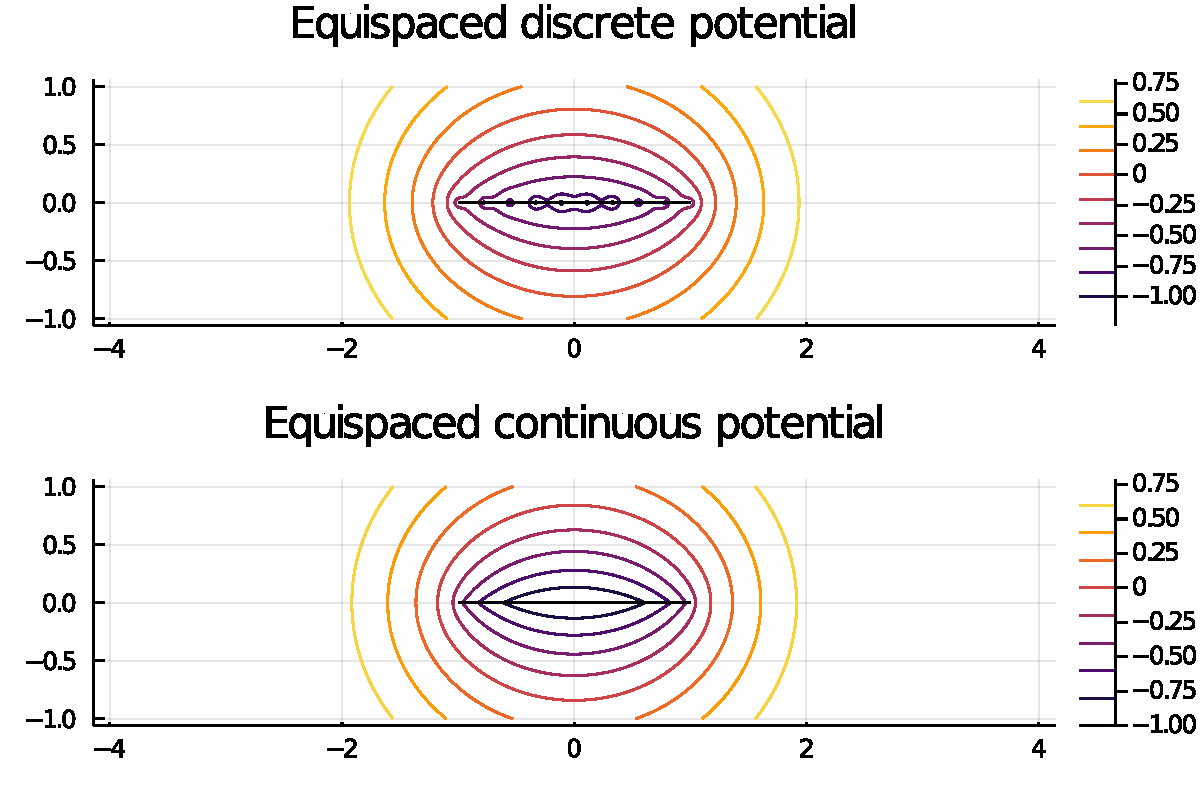
\includegraphics[width=\linewidth]{C:/Users/mfaso/OneDrive/Documents/GitHub/M3M6AppliedComplexAnalysis/output/figures/MasteryMaterial_15_1.pdf}

\begin{lstlisting}
(*@\HLJLn{\ensuremath{\phi}}@*) (*@\HLJLoB{=}@*) (*@\HLJLn{z}@*) (*@\HLJLoB{->}@*) (*@\HLJLnf{real}@*)(*@\HLJLp{(}@*)(*@\HLJLni{2}@*)(*@\HLJLnf{log}@*)(*@\HLJLp{(}@*)(*@\HLJLnf{sqrt}@*)(*@\HLJLp{(}@*)(*@\HLJLn{z}@*)(*@\HLJLoB{-}@*)(*@\HLJLni{1}@*)(*@\HLJLp{)}@*) (*@\HLJLoB{+}@*) (*@\HLJLnf{sqrt}@*)(*@\HLJLp{(}@*)(*@\HLJLn{z}@*)(*@\HLJLoB{+}@*)(*@\HLJLni{1}@*)(*@\HLJLp{))}@*) (*@\HLJLoB{-}@*) (*@\HLJLni{2}@*)(*@\HLJLnf{log}@*)(*@\HLJLp{(}@*)(*@\HLJLni{2}@*)(*@\HLJLp{))}@*)
(*@\HLJLn{p1}@*) (*@\HLJLoB{=}@*) (*@\HLJLnf{contour}@*)(*@\HLJLp{(}@*)(*@\HLJLn{x}@*)(*@\HLJLp{,}@*)(*@\HLJLn{y}@*)(*@\HLJLp{,}@*)(*@\HLJLn{log}@*)(*@\HLJLoB{.}@*)(*@\HLJLp{(}@*)(*@\HLJLn{abs}@*)(*@\HLJLoB{.}@*)(*@\HLJLp{(}@*)(*@\HLJLnf{\ensuremath{\ell}}@*)(*@\HLJLp{(}@*)(*@\HLJLn{z}@*)(*@\HLJLp{,}@*)(*@\HLJLn{xn}@*)(*@\HLJLp{)))}@*)(*@\HLJLoB{/}@*)(*@\HLJLn{n}@*)(*@\HLJLp{;}@*)(*@\HLJLn{ratio}@*) (*@\HLJLoB{=}@*) (*@\HLJLnfB{1.0}@*)(*@\HLJLp{,}@*)(*@\HLJLn{title}@*)(*@\HLJLoB{=}@*)(*@\HLJLs{"{}Chebyshev}@*) (*@\HLJLs{discrete}@*) (*@\HLJLs{potential"{}}@*)(*@\HLJLp{,}@*) (*@\HLJLn{levels}@*)(*@\HLJLoB{=}@*) (*@\HLJLoB{-}@*)(*@\HLJLni{1}@*)(*@\HLJLoB{:}@*)(*@\HLJLnfB{0.2}@*)(*@\HLJLoB{:}@*)(*@\HLJLnfB{0.6}@*)(*@\HLJLp{)}@*)
(*@\HLJLnf{plot!}@*)(*@\HLJLp{(}@*)(*@\HLJLoB{-}@*)(*@\HLJLnfB{1..1}@*)(*@\HLJLp{;}@*) (*@\HLJLn{color}@*)(*@\HLJLoB{=:}@*)(*@\HLJLn{black}@*)(*@\HLJLp{,}@*)(*@\HLJLn{label}@*)(*@\HLJLoB{=}@*)(*@\HLJLkc{false}@*)(*@\HLJLp{)}@*)
(*@\HLJLn{p2}@*) (*@\HLJLoB{=}@*) (*@\HLJLnf{contour}@*)(*@\HLJLp{(}@*)(*@\HLJLn{x}@*)(*@\HLJLp{,}@*)(*@\HLJLn{y}@*)(*@\HLJLp{,}@*)(*@\HLJLn{\ensuremath{\phi}}@*)(*@\HLJLoB{.}@*)(*@\HLJLp{(}@*)(*@\HLJLn{z}@*)(*@\HLJLp{);}@*)(*@\HLJLn{ratio}@*)(*@\HLJLoB{=}@*)(*@\HLJLnfB{1.0}@*)(*@\HLJLp{,}@*) (*@\HLJLn{levels}@*) (*@\HLJLoB{=}@*) (*@\HLJLoB{-}@*)(*@\HLJLni{1}@*)(*@\HLJLoB{:}@*)(*@\HLJLnfB{0.2}@*)(*@\HLJLoB{:}@*)(*@\HLJLnfB{0.6}@*)(*@\HLJLp{,}@*) (*@\HLJLn{title}@*)(*@\HLJLoB{=}@*)(*@\HLJLs{"{}Chebyshev}@*) (*@\HLJLs{continuous}@*) (*@\HLJLs{potential"{}}@*)(*@\HLJLp{)}@*)
(*@\HLJLnf{plot!}@*)(*@\HLJLp{(}@*)(*@\HLJLoB{-}@*)(*@\HLJLnfB{1..1}@*)(*@\HLJLp{;}@*) (*@\HLJLn{color}@*)(*@\HLJLoB{=:}@*)(*@\HLJLn{black}@*)(*@\HLJLp{,}@*)(*@\HLJLn{label}@*)(*@\HLJLoB{=}@*)(*@\HLJLkc{false}@*)(*@\HLJLp{)}@*)
(*@\HLJLnf{plot}@*)(*@\HLJLp{(}@*)(*@\HLJLn{p1}@*)(*@\HLJLp{,}@*)(*@\HLJLn{p2}@*)(*@\HLJLp{,}@*)(*@\HLJLn{layout}@*)(*@\HLJLoB{=}@*)(*@\HLJLp{(}@*)(*@\HLJLni{2}@*)(*@\HLJLp{,}@*)(*@\HLJLni{1}@*)(*@\HLJLp{))}@*)
\end{lstlisting}

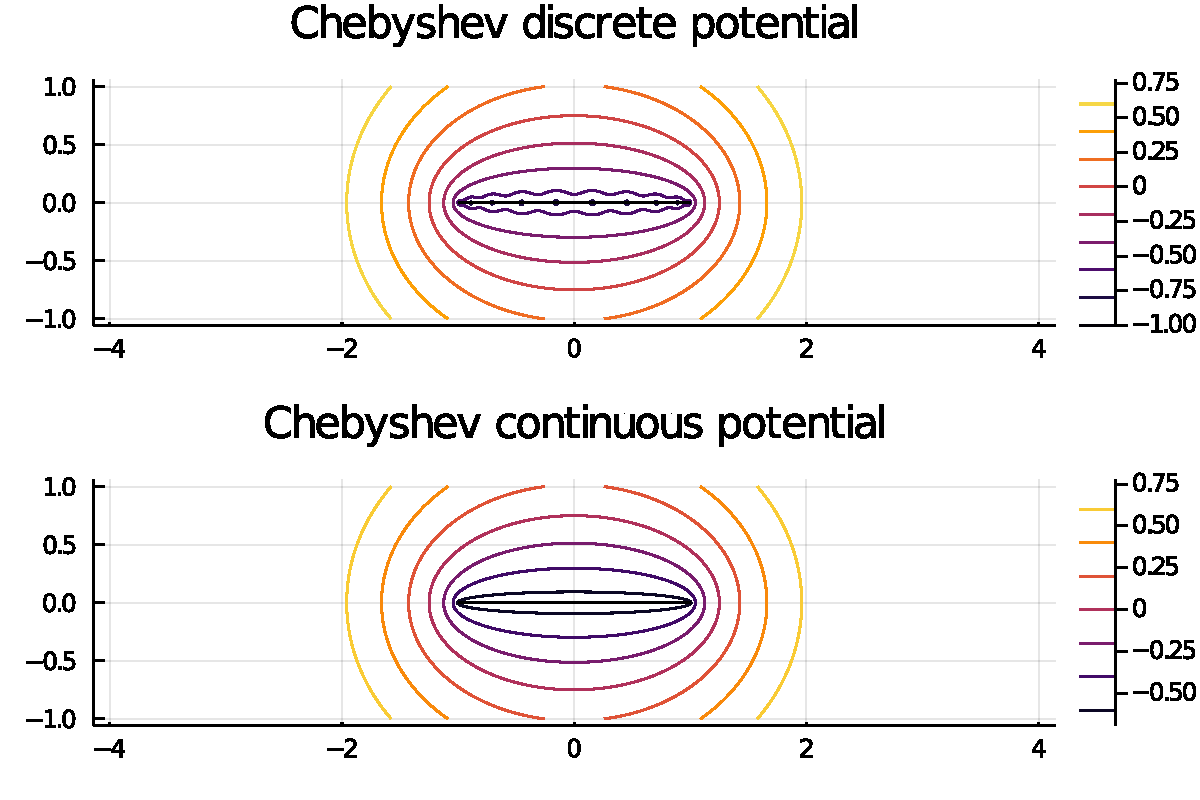
\includegraphics[width=\linewidth]{C:/Users/mfaso/OneDrive/Documents/GitHub/M3M6AppliedComplexAnalysis/output/figures/MasteryMaterial_16_1.pdf}

\textbf{Theorem (convergence/divergence on equipotential curves)} The interpolant $p_n(z)$ converges to $f(z)$ inside the largest equipotential curve of $\phi(z)$ that does not enclose any singularity of $f(z)$ and it diverges outside that curve. The asymptotic rate of converge or divergence is

\[
\left\vert f(z) - p_n(z)  \right\vert^{1/n} = \mathcal{O}\left( \exp\left(\phi(z) - \phi(z_0) \right)\right), \qquad n \to \infty,
\]
where $z_0$ is the location of the singularity of $f(z)$ that is closest to the interpolation interval $[-1, 1]$.

\textbf{Sketch of Proof} Recall the error bound

\[
\vert f(z) - p_n(z) \vert \leq  \left\lbrace\sup_{t \in \Gamma} \left\vert {\ell(z)\over\ell(t)} \right\vert\right\rbrace {1 \over 2\pi}  \oint_{\Gamma} \left\vert{f(t)\over t-z} \right\vert \dt,
\]
and the expression

\[
\left\vert {\ell(z)\over\ell(t)} \right\vert =  \exp\left[ n\left(\phi_n(z) - \phi_n(t) \right) \right].
\]
If we choose $\Gamma$ to be an equipotential curve that does not enclose the singularity at $z_0$ and $z$ lies inside $\Gamma$, then

\[
\left\vert {\ell(z)\over\ell(t)} \right\vert^{1/n} =  \exp\left[ \left(\phi_n(z) - \phi_n(t) \right) \right] \to \exp\left[ \left(\phi(z) - \phi(t) \right) \right], \qquad n\to \infty.
\]
Since $z$ is inside $\Gamma$, $t\in \Gamma$ and $\Gamma$ does not enclose $z_0$, $\phi(z) < \phi(t) < \phi(z_0)$ and thus the interpolant converges to $f$ at the stated rate.

Recall that the contour integral representation of $p_n(z)$ is still valid even if $z$ is outside $\Gamma$

\[
p_n(z) = {1 \over 2\pi\I} \oint_{\Gamma} {f(t)(\ell(t) - \ell(z))\over \ell(t)(t - z)}\dt.
\]
For the case where $z$ is outside $\Gamma$ but $\Gamma$ still does not enclose the singularity at $z_0$, the above formula simplifies to

\[
p_n(z) = {1 \over 2\pi\I} \oint_{\Gamma} {\ell(z)\over\ell(t)}   {f(t)\over(z - t)}\dt.
\]
Hence for large $n$ the magnitude of $p_n(z)$ behaves as

\[
\left\vert {\ell(z)\over\ell(t)} \right\vert \approx \exp\left[ n\left(\phi(z) - \phi(t) \right) \right]
\]
This is exponential growth since $z$ is outside $\Gamma$, which implies that $\phi(z) > \phi(t)$. If $f$ is bounded at $z$, the geometric growth of $p_n(z)$ with $n$ will dominate and $\vert f(z) - p_n(z) \vert$ will grow exponentially at a rate that is bounded by a constant times $\exp\left(n(\phi(z) - \phi(z_0)) \right)$. \ensuremath{\blacksquare}

We first examine the equipotential curves of the Chebyshev logarithmic potential function

\[
\phi(z) =  \Re \left\lbrace 2\log(\sqrt{z-1} + \sqrt{z+1})  \right\rbrace  -2 \log 2.
\]
If we set

\[
w = {1 \over 2}\left( \sqrt{z-1} + \sqrt{z+1} \right)^2,
\]
then we find that a circle in the $w$-plane of radius $\rho \geq 1$ is mapped to a Bernstein ellipse $E_{\rho}$ in the $z$-plane and $w$ is related to $\phi$ as follows

\[
\log\vert w \vert = \phi(z) + \log 2.
\]
This implies that the equipotential curves of $\phi$ are all Bernstein ellipses and if $\vert w \vert = \rho$, then

\[
\phi(z) = \log \rho - \log 2, \qquad z \in E_{\rho}.
\]
The interval $[-1, 1]$ is itself a degenerate Bernstein ellipse with $\rho = 1$ (and hence an equipotential curve) on which $\phi$ takes the value

\[
\phi(x) = -\log 2, \qquad x \in [-1, 1],
\]
as we showed in Lecture 16. Thus for $x$ on the unit interval and $z$ on a Bernstein ellipse,

\[
\phi(x) - \phi(z) = -\log 2 - (\log \rho - \log 2) = - \log \rho, \qquad x \in [-1, 1], z \in E_{\rho}.
\]
Combining this with the theorem we just proved, we conclude that if a function is analytic on and inside a Bernstein ellipse $E_{\rho}$, then Chebyshev interpolants converge at the rate

\[
\mathcal{O}\left( \rho^{-n} \right).
\]
In Lecture 19 we proved the same result for truncated Chebyshev expansions.

The Chebyshev measure $\mu(x) = 1/(\pi\sqrt{1-x^2})$ is special in the sense that it  is the unique measure that renders the logarithmic potential  $\phi$ constant on $[-1,1]$ and is therefore called the equilibrium measure. The electrostatic interpretation is that $\mu(x)$ is the unit charge distribution on $[-1, 1]$ that results in a constant electrostatic potential on $[-1, 1]$. This implies that the electric field vanishes on $[-1, 1]$, so there is no net force acting on the charges on $[-1, 1]$, hence the charges are in equilibrium. The configuration of charges according to the density $\mu(x)$ minimizes the energy of the system.

For Chebyshev interpolants to converge on $[-1, 1]$, a function just needs to be analytic on $[-1, 1]$ (i.e., a neighbourhood of $[-1, 1]$). For equally spaced interpolants to converge on $[-1, 1]$, the function has to be analytic on and inside the following much larger, eye-shaped region:


\begin{lstlisting}
(*@\HLJLn{\ensuremath{\phi}}@*) (*@\HLJLoB{=}@*) (*@\HLJLn{z}@*) (*@\HLJLoB{->}@*) (*@\HLJLnf{real}@*)(*@\HLJLp{((}@*)(*@\HLJLni{1}@*)(*@\HLJLoB{-}@*)(*@\HLJLn{z}@*)(*@\HLJLp{)}@*)(*@\HLJLoB{*}@*)(*@\HLJLnf{log}@*)(*@\HLJLp{(}@*)(*@\HLJLn{z}@*)(*@\HLJLoB{-}@*)(*@\HLJLni{1}@*)(*@\HLJLp{)}@*)(*@\HLJLoB{/}@*)(*@\HLJLni{2}@*) (*@\HLJLoB{+}@*) (*@\HLJLp{(}@*)(*@\HLJLni{1}@*)(*@\HLJLoB{+}@*)(*@\HLJLn{z}@*)(*@\HLJLp{)}@*)(*@\HLJLoB{*}@*)(*@\HLJLnf{log}@*)(*@\HLJLp{(}@*)(*@\HLJLn{z}@*)(*@\HLJLoB{+}@*)(*@\HLJLni{1}@*)(*@\HLJLp{)}@*)(*@\HLJLoB{/}@*)(*@\HLJLni{2}@*)(*@\HLJLp{)}@*) (*@\HLJLoB{-}@*) (*@\HLJLni{1}@*)
(*@\HLJLnf{contour}@*)(*@\HLJLp{(}@*)(*@\HLJLn{x}@*)(*@\HLJLp{,}@*)(*@\HLJLn{y}@*)(*@\HLJLp{,}@*)(*@\HLJLn{\ensuremath{\phi}}@*)(*@\HLJLoB{.}@*)(*@\HLJLp{(}@*)(*@\HLJLn{z}@*)(*@\HLJLp{);}@*)(*@\HLJLn{ratio}@*)(*@\HLJLoB{=}@*)(*@\HLJLnfB{1.0}@*)(*@\HLJLp{,}@*) (*@\HLJLn{levels}@*) (*@\HLJLoB{=}@*)(*@\HLJLp{[}@*)(*@\HLJLnf{log}@*)(*@\HLJLp{(}@*)(*@\HLJLni{2}@*)(*@\HLJLp{)}@*)(*@\HLJLoB{-}@*)(*@\HLJLni{1}@*)(*@\HLJLp{],}@*) (*@\HLJLn{legend}@*) (*@\HLJLoB{=}@*) (*@\HLJLkc{false}@*)(*@\HLJLp{)}@*)
(*@\HLJLnf{plot!}@*)(*@\HLJLp{(}@*)(*@\HLJLoB{-}@*)(*@\HLJLnfB{1..1}@*)(*@\HLJLp{;}@*) (*@\HLJLn{color}@*)(*@\HLJLoB{=:}@*)(*@\HLJLn{black}@*)(*@\HLJLp{)}@*)
\end{lstlisting}

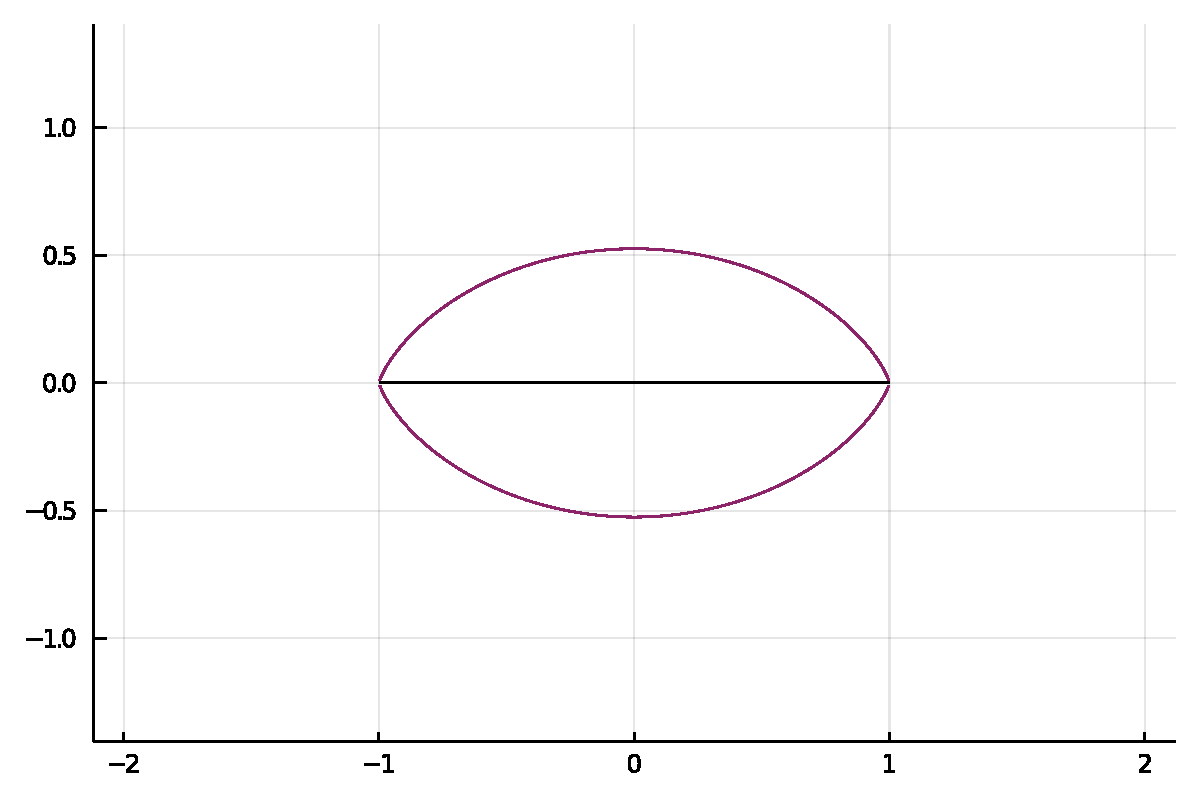
\includegraphics[width=\linewidth]{C:/Users/mfaso/OneDrive/Documents/GitHub/M3M6AppliedComplexAnalysis/output/figures/MasteryMaterial_17_1.pdf}

This region is the equipotential curve of the potential function for equally spaced points

\[
\Re \left\lbrace {1\over 2}(1-z) \log(z-1) + {1\over 2}(1+z) \log(z+1) \right\rbrace  -1
\]
that intersects the real axis at $x = \pm 1$.

\subsection{Example}
We take again the function $f = 1/(25z^2 + 1)$ and consider the rate of convergence or divergence on $[-1, 1]$ for equally spaced and Chebyshev interpolation.

Since $f$ is analytic within a Bernstein ellipse $E_{\rho}$ with $\rho = (1 + \sqrt{26})/5$, we expect Chebyshev interpolants to converge to $f$ on $[-1, 1]$ at the rate $\mathcal{O}(p^{-n})$.


\begin{lstlisting}
(*@\HLJLn{xf}@*) (*@\HLJLoB{=}@*) (*@\HLJLoB{-}@*)(*@\HLJLni{1}@*)(*@\HLJLoB{:}@*)(*@\HLJLnfB{0.001}@*)(*@\HLJLoB{:}@*)(*@\HLJLni{1}@*)
(*@\HLJLn{nv}@*) (*@\HLJLoB{=}@*) (*@\HLJLni{1}@*)(*@\HLJLoB{:}@*)(*@\HLJLni{200}@*)
(*@\HLJLn{errors}@*) (*@\HLJLoB{=}@*) (*@\HLJLp{[}@*)(*@\HLJLnf{maximum}@*)(*@\HLJLp{(}@*)(*@\HLJLn{abs}@*)(*@\HLJLoB{.}@*)(*@\HLJLp{(}@*)(*@\HLJLn{f}@*)(*@\HLJLoB{.}@*)(*@\HLJLp{(}@*)(*@\HLJLn{xf}@*)(*@\HLJLp{)}@*) (*@\HLJLoB{-}@*) (*@\HLJLnf{Fun}@*)(*@\HLJLp{(}@*)(*@\HLJLn{f}@*)(*@\HLJLp{,}@*)(*@\HLJLn{S}@*)(*@\HLJLp{,}@*)(*@\HLJLn{k}@*)(*@\HLJLp{)}@*)(*@\HLJLoB{.}@*)(*@\HLJLp{(}@*)(*@\HLJLn{xf}@*)(*@\HLJLp{)))}@*) (*@\HLJLk{for}@*) (*@\HLJLn{k}@*) (*@\HLJLoB{=}@*) (*@\HLJLn{nv}@*)(*@\HLJLp{]}@*)
(*@\HLJLnf{scatter}@*)(*@\HLJLp{(}@*)(*@\HLJLn{nv}@*)(*@\HLJLp{,}@*)(*@\HLJLn{errors}@*)(*@\HLJLp{;}@*)(*@\HLJLn{yscale}@*)(*@\HLJLoB{=:}@*)(*@\HLJLn{log10}@*)(*@\HLJLp{,}@*)(*@\HLJLn{ylabel}@*)(*@\HLJLoB{=}@*)(*@\HLJLs{"{}Error"{}}@*)(*@\HLJLp{,}@*)(*@\HLJLn{label}@*)(*@\HLJLoB{=}@*)(*@\HLJLs{"{}Chebyshev}@*) (*@\HLJLs{interpolation"{}}@*)(*@\HLJLp{)}@*)
(*@\HLJLn{\ensuremath{\rho}}@*) (*@\HLJLoB{=}@*) (*@\HLJLp{(}@*)(*@\HLJLni{1}@*)(*@\HLJLoB{+}@*)(*@\HLJLnf{sqrt}@*)(*@\HLJLp{(}@*)(*@\HLJLni{26}@*)(*@\HLJLp{))}@*)(*@\HLJLoB{/}@*)(*@\HLJLni{5}@*)
(*@\HLJLnf{plot!}@*)(*@\HLJLp{(}@*)(*@\HLJLn{nv}@*)(*@\HLJLp{,}@*)(*@\HLJLn{\ensuremath{\rho}}@*)(*@\HLJLoB{.{\textasciicircum}}@*)(*@\HLJLp{(}@*)(*@\HLJLoB{-}@*)(*@\HLJLn{nv}@*)(*@\HLJLp{);}@*)(*@\HLJLn{label}@*)(*@\HLJLoB{=}@*)(*@\HLJLs{"{}convergence}@*) (*@\HLJLs{estimate"{}}@*)(*@\HLJLp{)}@*)
\end{lstlisting}

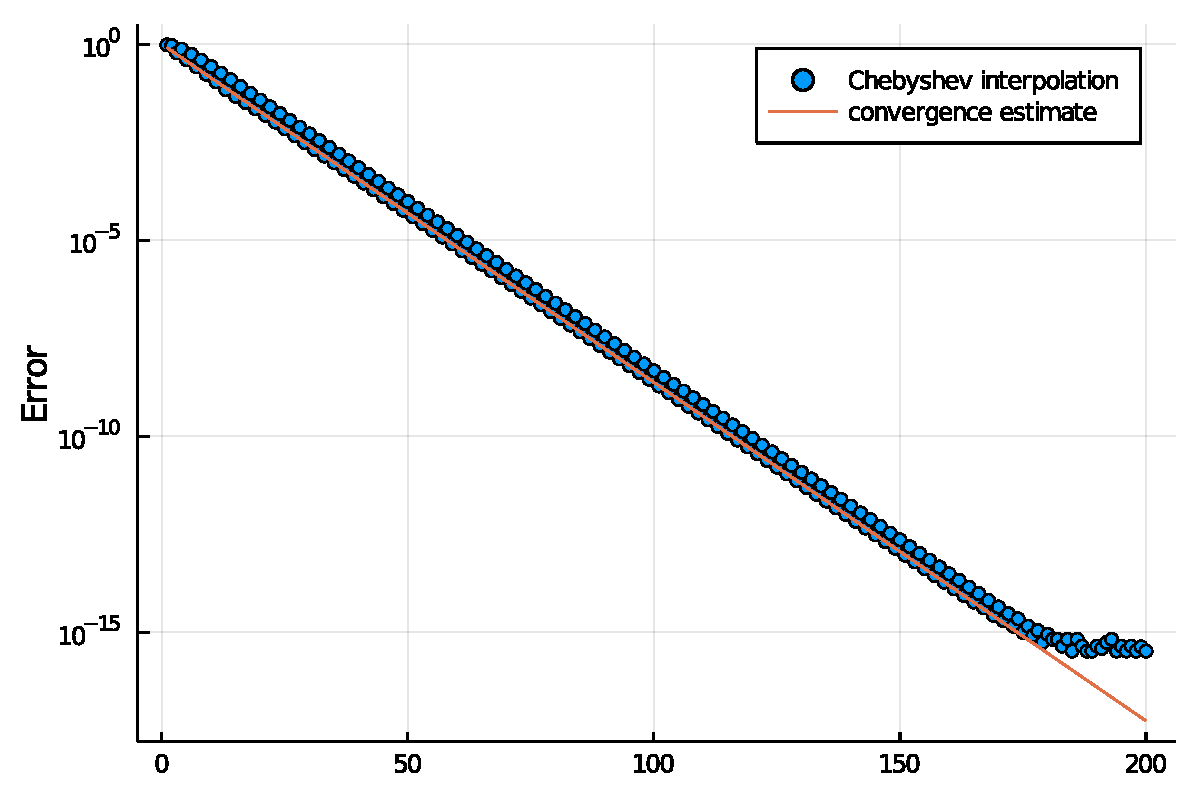
\includegraphics[width=\linewidth]{C:/Users/mfaso/OneDrive/Documents/GitHub/M3M6AppliedComplexAnalysis/output/figures/MasteryMaterial_18_1.pdf}

We know that equispaced interpolants won't converge to $f$ on $[-1, 1]$ since $f$ is not analytic in the eye-shaped region plotted above. According to the theorem above, the rate of convergence or divergence on $[-1, 1]$ hinges on the value of

\[
\phi(x) - \phi(\I/5) = {1\over 2}(1-x) \log(1-x) +  {1\over 2}(1+x) \log(1+x) - {1\over 2}\log\left({26\over25}\right)+{1\over5}\arctan(1/5)-{\pi\over10}.
\]
Here we check the formula is correct:


\begin{lstlisting}
(*@\HLJLn{\ensuremath{\delta}\ensuremath{\phi}}@*) (*@\HLJLoB{=}@*) (*@\HLJLn{x}@*) (*@\HLJLoB{->}@*) (*@\HLJLp{(}@*)(*@\HLJLni{1}@*)(*@\HLJLoB{-}@*)(*@\HLJLn{x}@*)(*@\HLJLp{)}@*)(*@\HLJLoB{/}@*)(*@\HLJLni{2}@*)(*@\HLJLoB{*}@*)(*@\HLJLnf{log}@*)(*@\HLJLp{(}@*)(*@\HLJLni{1}@*)(*@\HLJLoB{-}@*)(*@\HLJLn{x}@*)(*@\HLJLp{)}@*)(*@\HLJLoB{+}@*)(*@\HLJLp{(}@*)(*@\HLJLni{1}@*)(*@\HLJLoB{+}@*)(*@\HLJLn{x}@*)(*@\HLJLp{)}@*)(*@\HLJLoB{/}@*)(*@\HLJLni{2}@*)(*@\HLJLoB{*}@*)(*@\HLJLnf{log}@*)(*@\HLJLp{(}@*)(*@\HLJLni{1}@*)(*@\HLJLoB{+}@*)(*@\HLJLn{x}@*)(*@\HLJLp{)}@*) (*@\HLJLoB{-}@*) (*@\HLJLnf{log}@*)(*@\HLJLp{(}@*)(*@\HLJLni{26}@*)(*@\HLJLoB{/}@*)(*@\HLJLni{25}@*)(*@\HLJLp{)}@*)(*@\HLJLoB{/}@*)(*@\HLJLni{2}@*)(*@\HLJLoB{+}@*)(*@\HLJLnf{atan}@*)(*@\HLJLp{(}@*)(*@\HLJLni{1}@*)(*@\HLJLoB{/}@*)(*@\HLJLni{5}@*)(*@\HLJLp{)}@*)(*@\HLJLoB{/}@*)(*@\HLJLni{5}@*)(*@\HLJLoB{-}@*)(*@\HLJLn{\ensuremath{\pi}}@*)(*@\HLJLoB{/}@*)(*@\HLJLni{10}@*)
(*@\HLJLn{x}@*) (*@\HLJLoB{=}@*) (*@\HLJLnfB{0.2}@*)
(*@\HLJLnf{\ensuremath{\phi}}@*)(*@\HLJLp{(}@*)(*@\HLJLn{x}@*)(*@\HLJLoB{+}@*)(*@\HLJLnfB{0.0}@*)(*@\HLJLn{im}@*)(*@\HLJLp{)}@*) (*@\HLJLoB{-}@*) (*@\HLJLnf{\ensuremath{\phi}}@*)(*@\HLJLp{(}@*)(*@\HLJLn{im}@*)(*@\HLJLoB{/}@*)(*@\HLJLni{5}@*)(*@\HLJLp{),}@*) (*@\HLJLnf{\ensuremath{\delta}\ensuremath{\phi}}@*)(*@\HLJLp{(}@*)(*@\HLJLn{x}@*)(*@\HLJLp{)}@*)
\end{lstlisting}

\begin{lstlisting}
(-0.274154996414955, -0.27415499641495494)
\end{lstlisting}


Here is a plot of $\phi(x) - \phi(\I/5)$:


\begin{lstlisting}
(*@\HLJLn{\ensuremath{\delta}\ensuremath{\phi}}@*) (*@\HLJLoB{=}@*) (*@\HLJLnf{Fun}@*)(*@\HLJLp{(}@*)(*@\HLJLn{\ensuremath{\delta}\ensuremath{\phi}}@*)(*@\HLJLp{,}@*)(*@\HLJLnf{Chebyshev}@*)(*@\HLJLp{())}@*)
(*@\HLJLnf{plot}@*)(*@\HLJLp{(}@*)(*@\HLJLn{\ensuremath{\delta}\ensuremath{\phi}}@*)(*@\HLJLp{;}@*)(*@\HLJLn{legend}@*)(*@\HLJLoB{=}@*)(*@\HLJLkc{false}@*)(*@\HLJLp{)}@*)
\end{lstlisting}

\includegraphics[width=\linewidth]{C:/Users/mfaso/OneDrive/Documents/GitHub/M3M6AppliedComplexAnalysis/output/figures/MasteryMaterial_20_1.pdf}

We expect equispaced interpolants to converge where $\phi(x) - \phi(\I/5) < 0$ and diverge where $\phi(x) - \phi(\I/5) > 0$. Moreover, the interpolant converges fastest at $x=0$ (as $\exp\left[n(\phi(0) - \phi(\I/5)) \right]$) and diverges fastest at $x = \pm 1$ (as $\exp\left[n(\phi(\pm 1) - \phi(\I/5)) \right]$).


\begin{lstlisting}
(*@\HLJLnf{roots}@*)(*@\HLJLp{(}@*)(*@\HLJLn{\ensuremath{\delta}\ensuremath{\phi}}@*)(*@\HLJLp{)}@*)
\end{lstlisting}

\begin{lstlisting}
2-element Array(*@{{\{}}@*)Float64,1(*@{{\}}}@*):
 -0.7266768604776661
  0.7266768604776662
\end{lstlisting}


\begin{lstlisting}
(*@\HLJLn{nv}@*) (*@\HLJLoB{=}@*) (*@\HLJLni{2}@*)(*@\HLJLoB{:}@*)(*@\HLJLni{200}@*)
(*@\HLJLn{errors}@*) (*@\HLJLoB{=}@*) (*@\HLJLp{[}@*)(*@\HLJLnf{maximum}@*)(*@\HLJLp{(}@*)(*@\HLJLn{abs}@*)(*@\HLJLoB{.}@*)(*@\HLJLp{(}@*)(*@\HLJLn{f}@*)(*@\HLJLoB{.}@*)(*@\HLJLp{(}@*)(*@\HLJLn{xf}@*)(*@\HLJLp{)}@*) (*@\HLJLoB{-}@*) (*@\HLJLnf{equi{\_}interp}@*)(*@\HLJLp{(}@*)(*@\HLJLn{f}@*)(*@\HLJLp{,}@*)(*@\HLJLn{k}@*)(*@\HLJLp{)}@*)(*@\HLJLoB{.}@*)(*@\HLJLp{(}@*)(*@\HLJLn{xf}@*)(*@\HLJLp{)))}@*) (*@\HLJLk{for}@*) (*@\HLJLn{k}@*) (*@\HLJLoB{=}@*) (*@\HLJLn{nv}@*)(*@\HLJLp{]}@*)
(*@\HLJLnf{scatter}@*)(*@\HLJLp{(}@*)(*@\HLJLn{nv}@*)(*@\HLJLp{,}@*)(*@\HLJLn{errors}@*)(*@\HLJLp{;}@*)(*@\HLJLn{yscale}@*)(*@\HLJLoB{=:}@*)(*@\HLJLn{log10}@*)(*@\HLJLp{,}@*)(*@\HLJLn{label}@*)(*@\HLJLoB{=}@*)(*@\HLJLs{"{}Equispaced}@*) (*@\HLJLs{interpolation}@*) (*@\HLJLs{error}@*) (*@\HLJLs{on}@*) (*@\HLJLs{[-1,}@*) (*@\HLJLs{1]"{}}@*)(*@\HLJLp{)}@*)
(*@\HLJLnf{plot!}@*)(*@\HLJLp{(}@*)(*@\HLJLni{1}@*)(*@\HLJLoB{:}@*)(*@\HLJLni{50}@*)(*@\HLJLp{,}@*)(*@\HLJLn{exp}@*)(*@\HLJLoB{.}@*)(*@\HLJLp{((}@*)(*@\HLJLni{1}@*)(*@\HLJLoB{:}@*)(*@\HLJLni{50}@*)(*@\HLJLp{)}@*)(*@\HLJLoB{*}@*)(*@\HLJLnf{\ensuremath{\delta}\ensuremath{\phi}}@*)(*@\HLJLp{(}@*)(*@\HLJLni{1}@*)(*@\HLJLp{));}@*)(*@\HLJLn{label}@*)(*@\HLJLoB{=}@*)(*@\HLJLs{"{}divergence}@*) (*@\HLJLs{estimate"{}}@*)(*@\HLJLp{)}@*)
(*@\HLJLn{err0}@*) (*@\HLJLoB{=}@*) (*@\HLJLp{[}@*)(*@\HLJLnf{abs}@*)(*@\HLJLp{(}@*)(*@\HLJLnf{f}@*)(*@\HLJLp{(}@*)(*@\HLJLni{0}@*)(*@\HLJLp{)}@*) (*@\HLJLoB{-}@*) (*@\HLJLnf{equi{\_}interp}@*)(*@\HLJLp{(}@*)(*@\HLJLn{f}@*)(*@\HLJLp{,}@*)(*@\HLJLn{k}@*)(*@\HLJLp{)(}@*)(*@\HLJLni{0}@*)(*@\HLJLp{))}@*) (*@\HLJLk{for}@*) (*@\HLJLn{k}@*) (*@\HLJLoB{=}@*) (*@\HLJLn{nv}@*)(*@\HLJLp{]}@*) (*@\HLJLcs{{\#}error}@*) (*@\HLJLcs{at}@*) (*@\HLJLcs{0}@*)
(*@\HLJLnf{scatter!}@*)(*@\HLJLp{(}@*)(*@\HLJLn{nv}@*)(*@\HLJLp{,}@*)(*@\HLJLn{err0}@*)(*@\HLJLoB{.+}@*)(*@\HLJLnf{eps}@*)(*@\HLJLp{();}@*)(*@\HLJLn{yscale}@*)(*@\HLJLoB{=:}@*)(*@\HLJLn{log10}@*)(*@\HLJLp{,}@*)(*@\HLJLn{label}@*)(*@\HLJLoB{=}@*)(*@\HLJLs{"{}equispaced}@*) (*@\HLJLs{interpolation}@*) (*@\HLJLs{error}@*) (*@\HLJLs{at}@*) (*@\HLJLs{0"{}}@*)(*@\HLJLp{)}@*)
(*@\HLJLnf{plot!}@*)(*@\HLJLp{(}@*)(*@\HLJLni{1}@*)(*@\HLJLoB{:}@*)(*@\HLJLni{100}@*)(*@\HLJLp{,}@*)(*@\HLJLn{exp}@*)(*@\HLJLoB{.}@*)(*@\HLJLp{((}@*)(*@\HLJLni{1}@*)(*@\HLJLoB{:}@*)(*@\HLJLni{100}@*)(*@\HLJLp{)}@*)(*@\HLJLoB{*}@*)(*@\HLJLnf{\ensuremath{\delta}\ensuremath{\phi}}@*)(*@\HLJLp{(}@*)(*@\HLJLni{0}@*)(*@\HLJLp{));}@*)(*@\HLJLn{label}@*)(*@\HLJLoB{=}@*)(*@\HLJLs{"{}convergence}@*) (*@\HLJLs{estimate"{}}@*)(*@\HLJLp{)}@*)
\end{lstlisting}

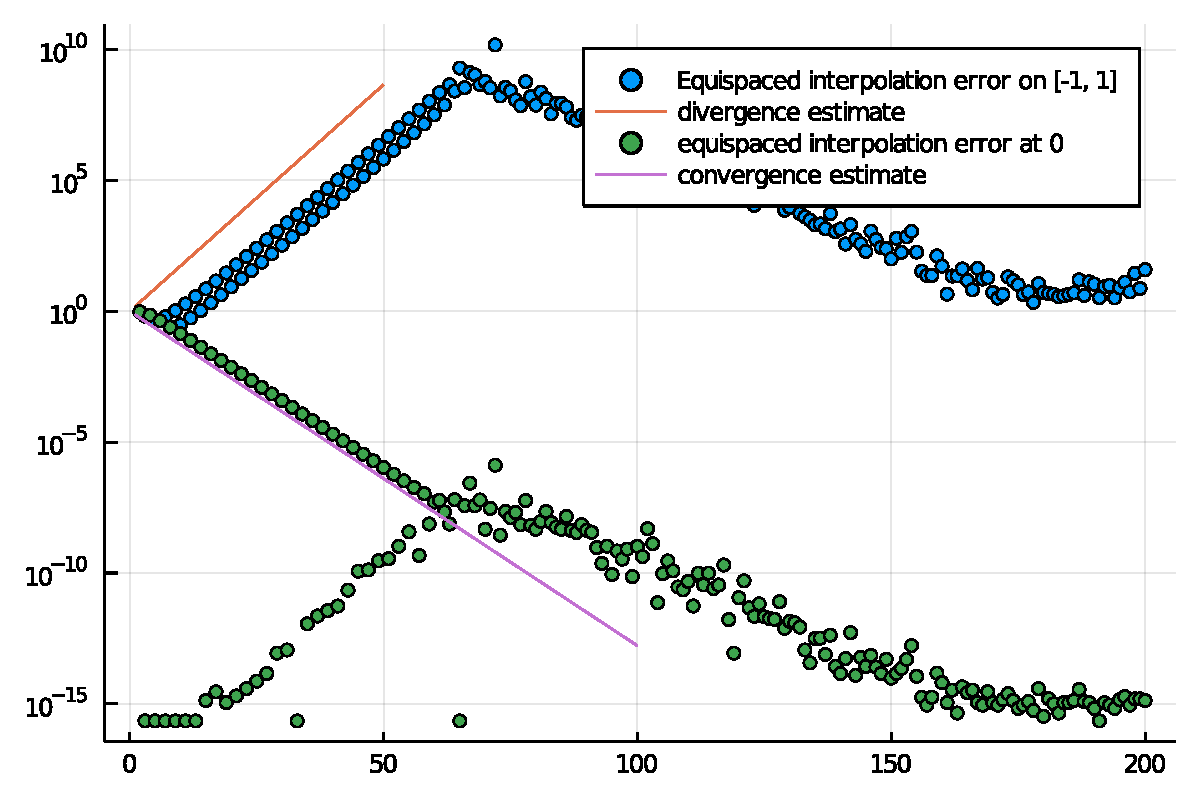
\includegraphics[width=\linewidth]{C:/Users/mfaso/OneDrive/Documents/GitHub/M3M6AppliedComplexAnalysis/output/figures/MasteryMaterial_22_1.pdf}

The interpolant converges and diverges at the predicted rates but at $n \approx 60$ the rates slow down because interpolation at equally spaced points is numerically unstable.



\end{document}
